\documentclass{beamer}
\usetheme{metropolis}
\usepackage{graphicx}
\usepackage{subfig}
\usepackage{tcolorbox}
\title{Computer Logic and Digital Circuit Design (PHYS306/COSC330): Unit 1}
\author{Jordan Hanson}
\institute{Whittier College Department of Physics and Astronomy}

\begin{document}
\maketitle

\section{Summary}

\begin{frame}{Unit 1 Summary - Theoretical Logic Gates, and Operations}
\begin{enumerate}
\item Logic Gates
\begin{itemize}
\item Circuit diagram
\item Truth table
\item Timing diagram
\item Boolean logic
\end{itemize}
\item \alert{Boolean algebra I}
\item IC Circuits, \textbf{data sheets}
\item \alert{Boolean algebra II}
\end{enumerate}
\end{frame}

\section{Logic Gates}

\begin{frame}{Logic Gates}
A \textbf{logic gate} is a digital circuit component made of transistors, that performs a basic logic function with $n$ inputs and $m$ outputs. \\ \vspace{0.5cm}
\begin{columns}[T]
\begin{column}{0.5\textwidth}
We will cover this basic set:
\begin{itemize}
\item NOT, $n=1$, $m=1$
\item AND, $n$, $m=1$
\item OR, $n$, $m=1$
\item NAND, $n$, $m=1$
\item NOR, $n=2$, $m=1$
\item XOR, $n=2$, $m=1$
\item XNOR, $n=2$, $m=1$
\end{itemize}
\end{column}
\begin{column}{0.5\textwidth}
Each gate has $n$ inputs, and $m$ outputs.  We represent the inputs (HIGH/LOW) with $A$, $B$, ..., and the output usually with $X$. \\ \vspace{0.5cm}
\begin{itemize}
\item Circuit diagram
\item Truth table
\item Timing diagram
\item Boolean logic
\end{itemize}
\end{column}
\end{columns}
\end{frame}

\begin{frame}{Logic Gates}
\textbf{The NOT gate:} flips the input from LOW/HIGH to HIGH/LOW. \\ \vspace{0.5cm}
\begin{columns}[T]
\begin{column}{0.5\textwidth}
\begin{itemize}
\item \alert{NOT, $n=1$, $m=1$}
\item AND, $n$, $m=1$
\item OR, $n$, $m=1$
\item NAND, $n$, $m=1$
\item NOR, $n=2$, $m=1$
\item XOR, $n=2$, $m=1$
\item XNOR, $n=2$, $m=1$
\end{itemize}
\end{column}
\begin{column}{0.5\textwidth}
\begin{figure}
\centering
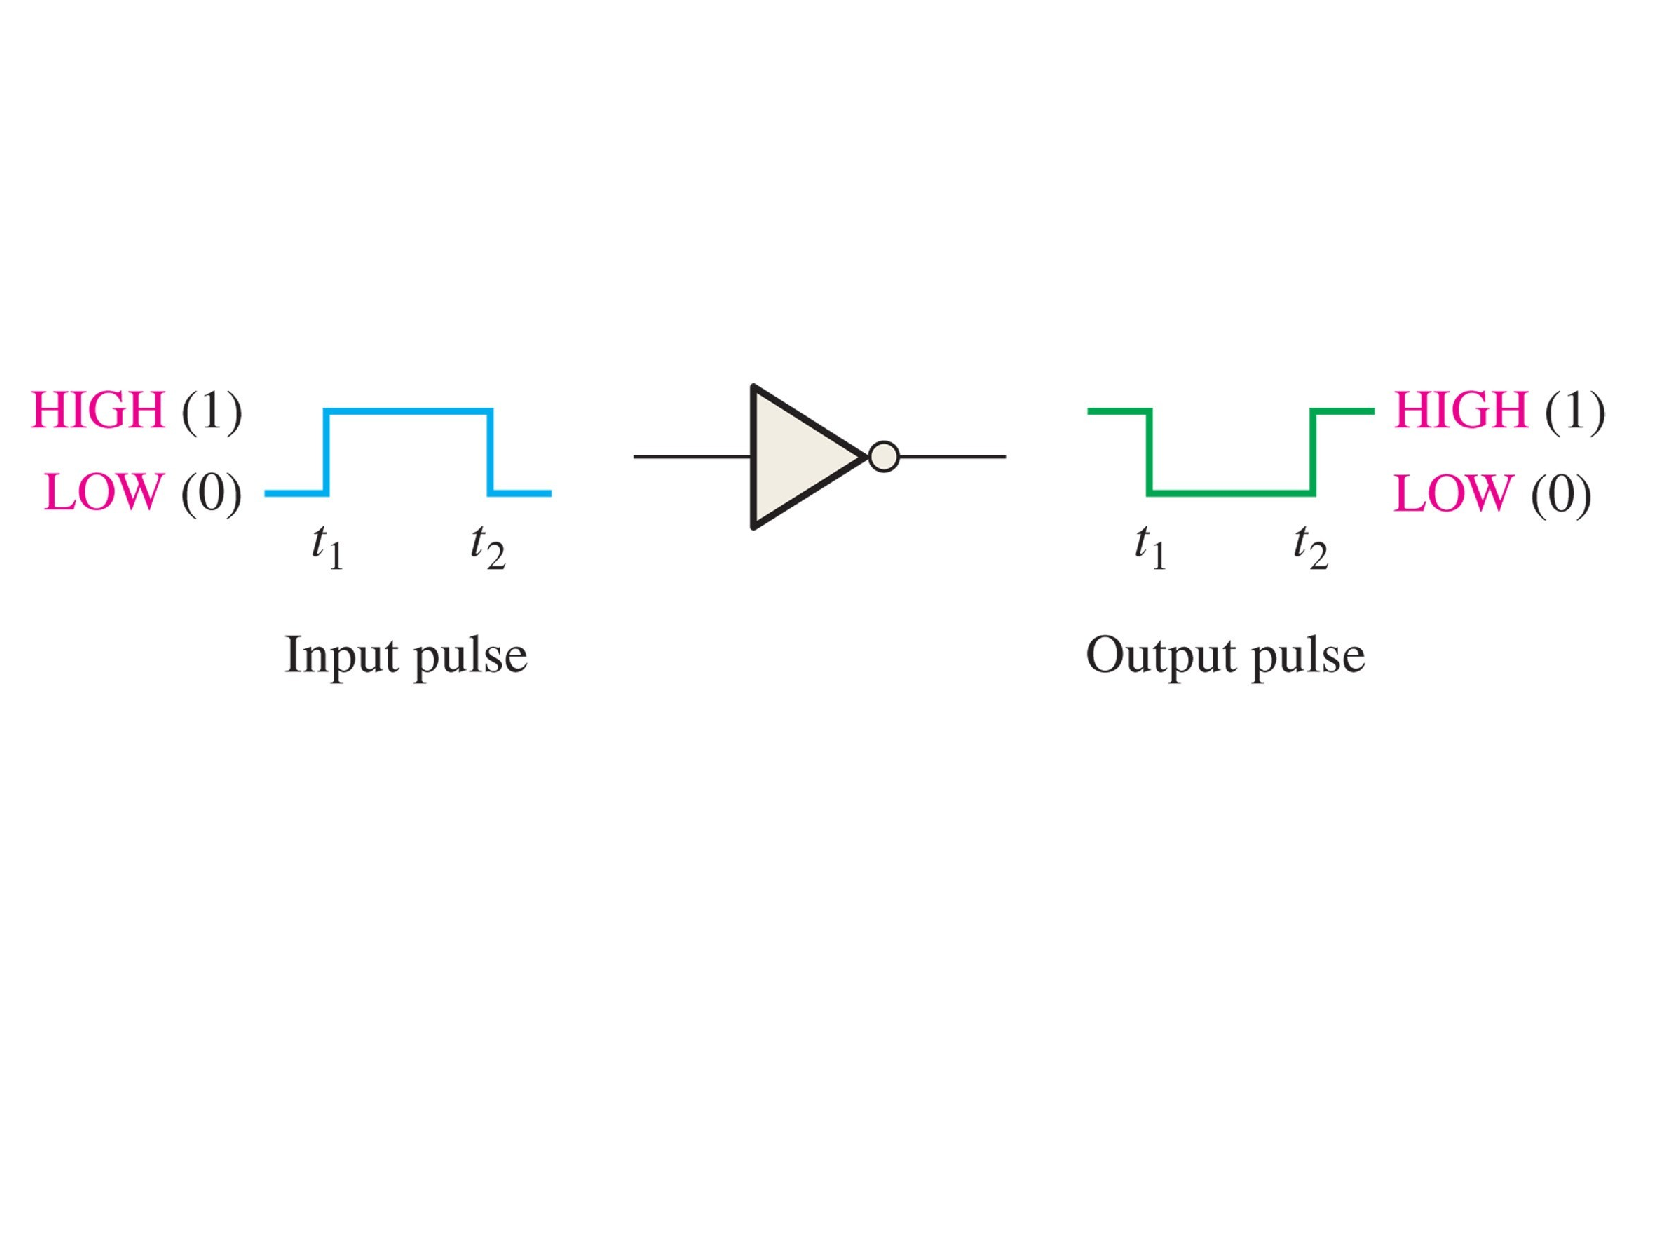
\includegraphics[width=0.9\textwidth,trim=0cm 6cm 0cm 4cm,clip=true]{figures/newNot.pdf}
\caption{\label{fig:not} The NOT gate is represented with a triangle and a circle.  It has one input and one output.}
\end{figure}
\end{column}
\end{columns}
\end{frame}

\begin{frame}{Logic Gates}
\textbf{The NOT gate:} flips the input from LOW/HIGH to HIGH/LOW. \\ \vspace{0.5cm}
\begin{columns}[T]
\begin{column}{0.5\textwidth}
\begin{itemize}
\item \alert{NOT, $n=1$, $m=1$}
\item AND, $n$, $m=1$
\item OR, $n$, $m=1$
\item NAND, $n$, $m=1$
\item NOR, $n=2$, $m=1$
\item XOR, $n=2$, $m=1$
\item XNOR, $n=2$, $m=1$
\end{itemize}
\end{column}
\begin{column}{0.5\textwidth}
\begin{table}
\begin{tabular}{c c}
IN & OUT \\
1 & 0 \\
0 & 1
\end{tabular}
\caption{\label{tab:NOT} Truth table for NOT.}
\end{table}
\end{column}
\end{columns}
\end{frame}

\begin{frame}{Logic Gates}
\textbf{The NOT gate:} flips the input from LOW/HIGH to HIGH/LOW. \\ \vspace{0.5cm}
\begin{columns}[T]
\begin{column}{0.5\textwidth}
\begin{itemize}
\item \alert{NOT, $n=1$, $m=1$}
\item AND, $n$, $m=1$
\item OR, $n$, $m=1$
\item NAND, $n$, $m=1$
\item NOR, $n=2$, $m=1$
\item XOR, $n=2$, $m=1$
\item XNOR, $n=2$, $m=1$
\end{itemize}
\end{column}
\begin{column}{0.5\textwidth}
\begin{figure}
\centering
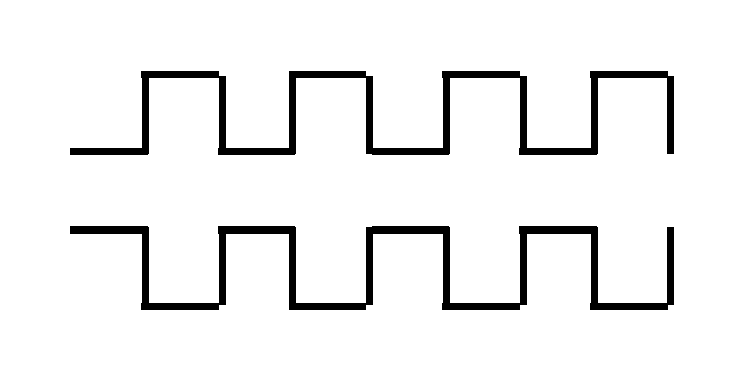
\includegraphics[width=0.8\textwidth]{figures/TimingNot.pdf}
\caption{\label{fig:not2} Example timing diagram for the NOT gate.  (Top) example signal, $s$.  (Bottom) NOT $s$, or $\bar{s}$.}
\end{figure}
\end{column}
\end{columns}
\end{frame}

\begin{frame}{Logic Gates}
\textbf{The NOT gate:} flips the input from LOW/HIGH to HIGH/LOW. \\ \vspace{0.5cm}
\begin{columns}[T]
\begin{column}{0.5\textwidth}
\begin{itemize}
\item \alert{NOT, $n=1$, $m=1$}
\item AND, $n$, $m=1$
\item OR, $n$, $m=1$
\item NAND, $n$, $m=1$
\item NOR, $n=2$, $m=1$
\item XOR, $n=2$, $m=1$
\item XNOR, $n=2$, $m=1$
\end{itemize}
\end{column}
\begin{column}{0.5\textwidth}
\begin{equation}
NOT (A) = \bar{A}
\end{equation}
\end{column}
\end{columns}
\end{frame}

\begin{frame}{Logic Gates}
\textbf{The NOT gate:} flips the input from LOW/HIGH to HIGH/LOW. \\ \vspace{0.5cm}
\begin{columns}[T]
\begin{column}{0.5\textwidth}
\begin{itemize}
\item \alert{NOT, $n=1$, $m=1$}
\item AND, $n$, $m=1$
\item OR, $n$, $m=1$
\item NAND, $n$, $m=1$
\item NOR, $n=2$, $m=1$
\item XOR, $n=2$, $m=1$
\item XNOR, $n=2$, $m=1$
\end{itemize}
\end{column}
\begin{column}{0.5\textwidth}
\textbf{In class exercises:}
\small
\begin{itemize}
\item Using NOT gates, create a circuit that forms the 2's compliment of an 8 bit binary number.
\item Once you have this, draw a timing diagram representing the conversion of 13 to the proper 1's compliment.
\end{itemize}
\end{column}
\end{columns}
\end{frame}

\begin{frame}{Logic Gates}
\textbf{The AND gate:} requires both inputs to be HIGH, for HIGH output. \\ \vspace{0.5cm}
\begin{columns}[T]
\begin{column}{0.5\textwidth}
\begin{itemize}
\item \alert{NOT, $n=1$, $m=1$}
\item \alert{AND, $n$, $m=1$}
\item OR, $n$, $m=1$
\item NAND, $n$, $m=1$
\item NOR, $n=2$, $m=1$
\item XOR, $n=2$, $m=1$
\item XNOR, $n=2$, $m=1$
\end{itemize}
\end{column}
\begin{column}{0.5\textwidth}
\begin{figure}
\centering
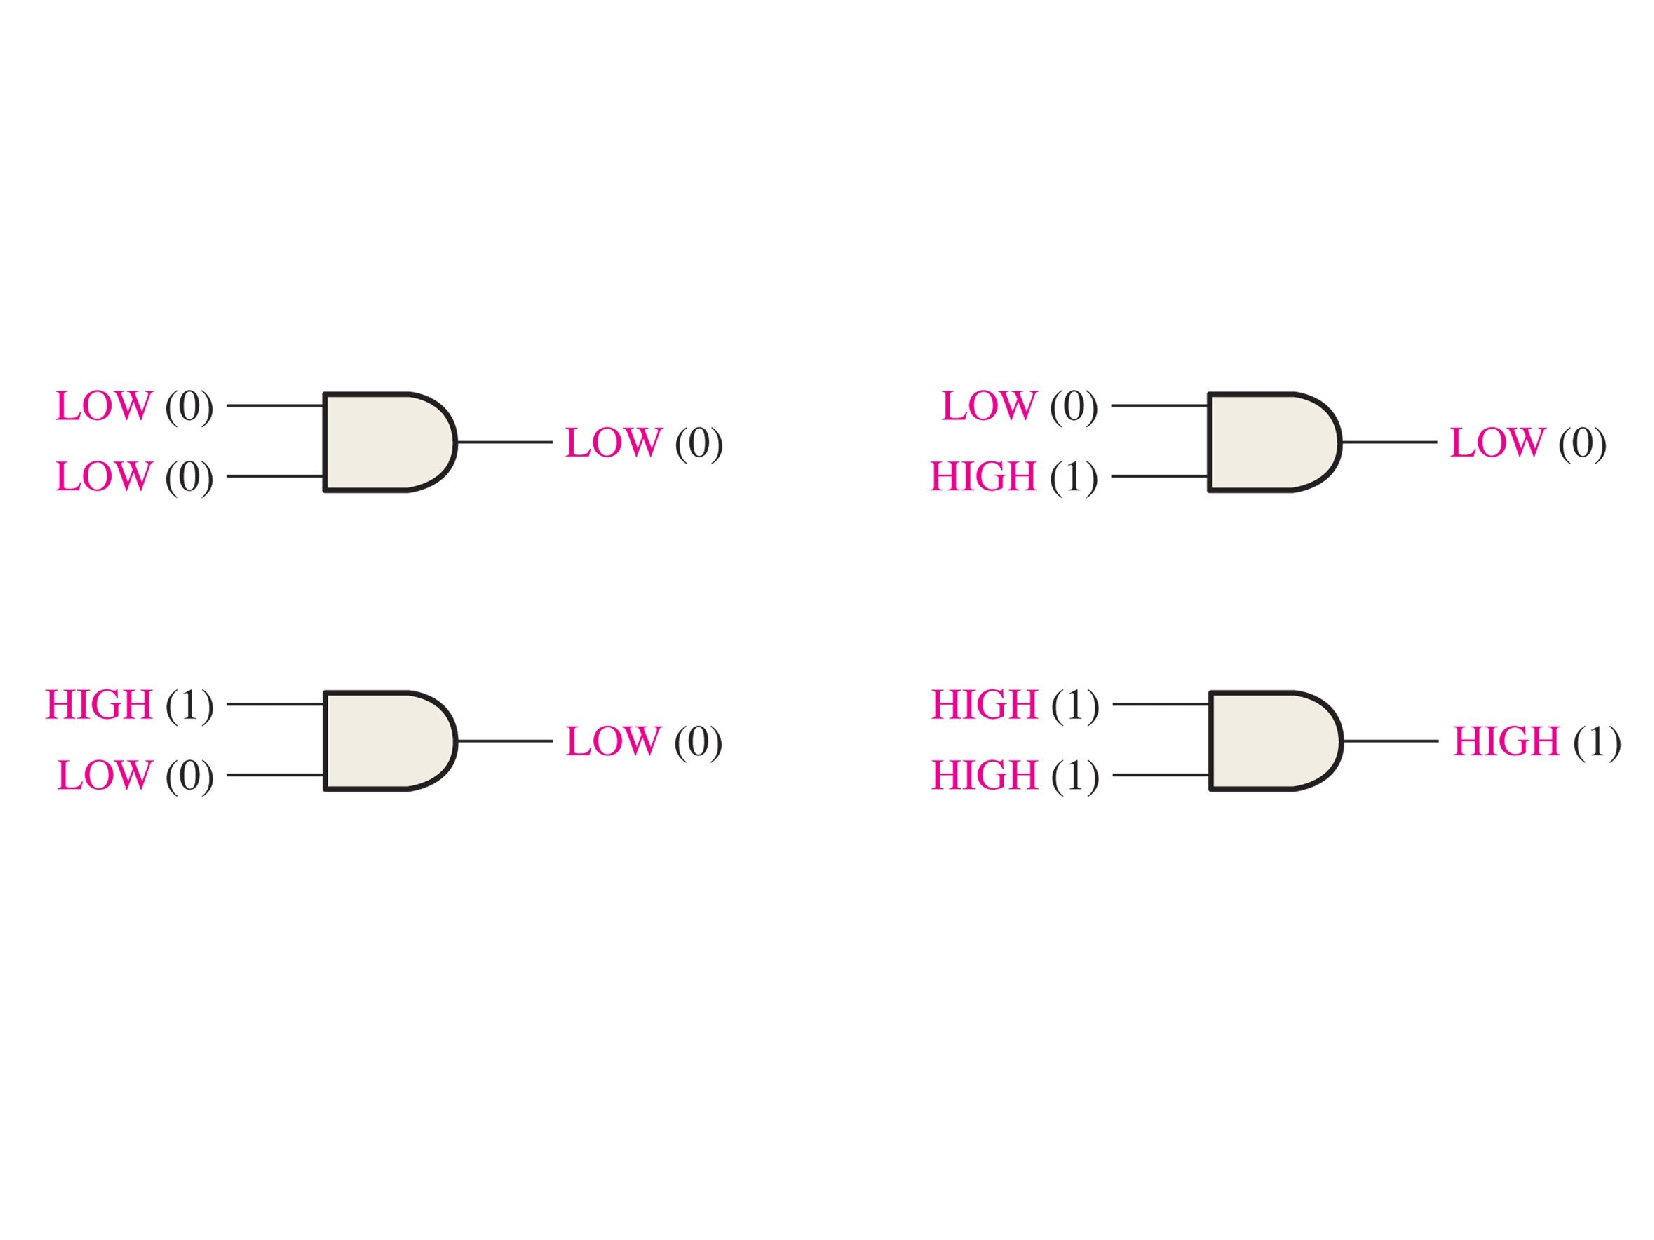
\includegraphics[width=0.9\textwidth,trim=0cm 5cm 0cm 5cm,clip=true]{figures/newAnd.pdf}
\caption{\label{fig:and} The circuit representation of an AND gate.  Two inputs, one output.}
\end{figure}
\end{column}
\end{columns}
\end{frame}

\begin{frame}{Logic Gates}
\textbf{The AND gate:} requires both inputs to be HIGH, for HIGH output. \\ \vspace{0.5cm}
\begin{columns}[T]
\begin{column}{0.5\textwidth}
\begin{itemize}
\item \alert{NOT, $n=1$, $m=1$}
\item \alert{AND, $n$, $m=1$}
\item OR, $n$, $m=1$
\item NAND, $n$, $m=1$
\item NOR, $n=2$, $m=1$
\item XOR, $n=2$, $m=1$
\item XNOR, $n=2$, $m=1$
\end{itemize}
\end{column}
\begin{column}{0.5\textwidth}
\begin{table}
\begin{tabular}{c c c}
A & B & X \\
1 & 1 & 1 \\
1 & 0 & 0 \\
0 & 1 & 0 \\
0 & 0 & 0
\end{tabular}
\caption{\label{tab:AND} Truth table for AND.}
\end{table}
\small 
How many input combinations are there for $n$?  Specifically, how many for two-input gates?  Three-input?
\end{column}
\end{columns}
\end{frame}

\begin{frame}{Logic Gates}
\textbf{The AND gate:} requires both inputs to be HIGH, for HIGH output. \\ \vspace{0.5cm}
\begin{columns}[T]
\begin{column}{0.5\textwidth}
\begin{itemize}
\item \alert{NOT, $n=1$, $m=1$}
\item \alert{AND, $n$, $m=1$}
\item OR, $n$, $m=1$
\item NAND, $n$, $m=1$
\item NOR, $n=2$, $m=1$
\item XOR, $n=2$, $m=1$
\item XNOR, $n=2$, $m=1$
\end{itemize}
\end{column}
\begin{column}{0.5\textwidth}
\begin{figure}
\centering
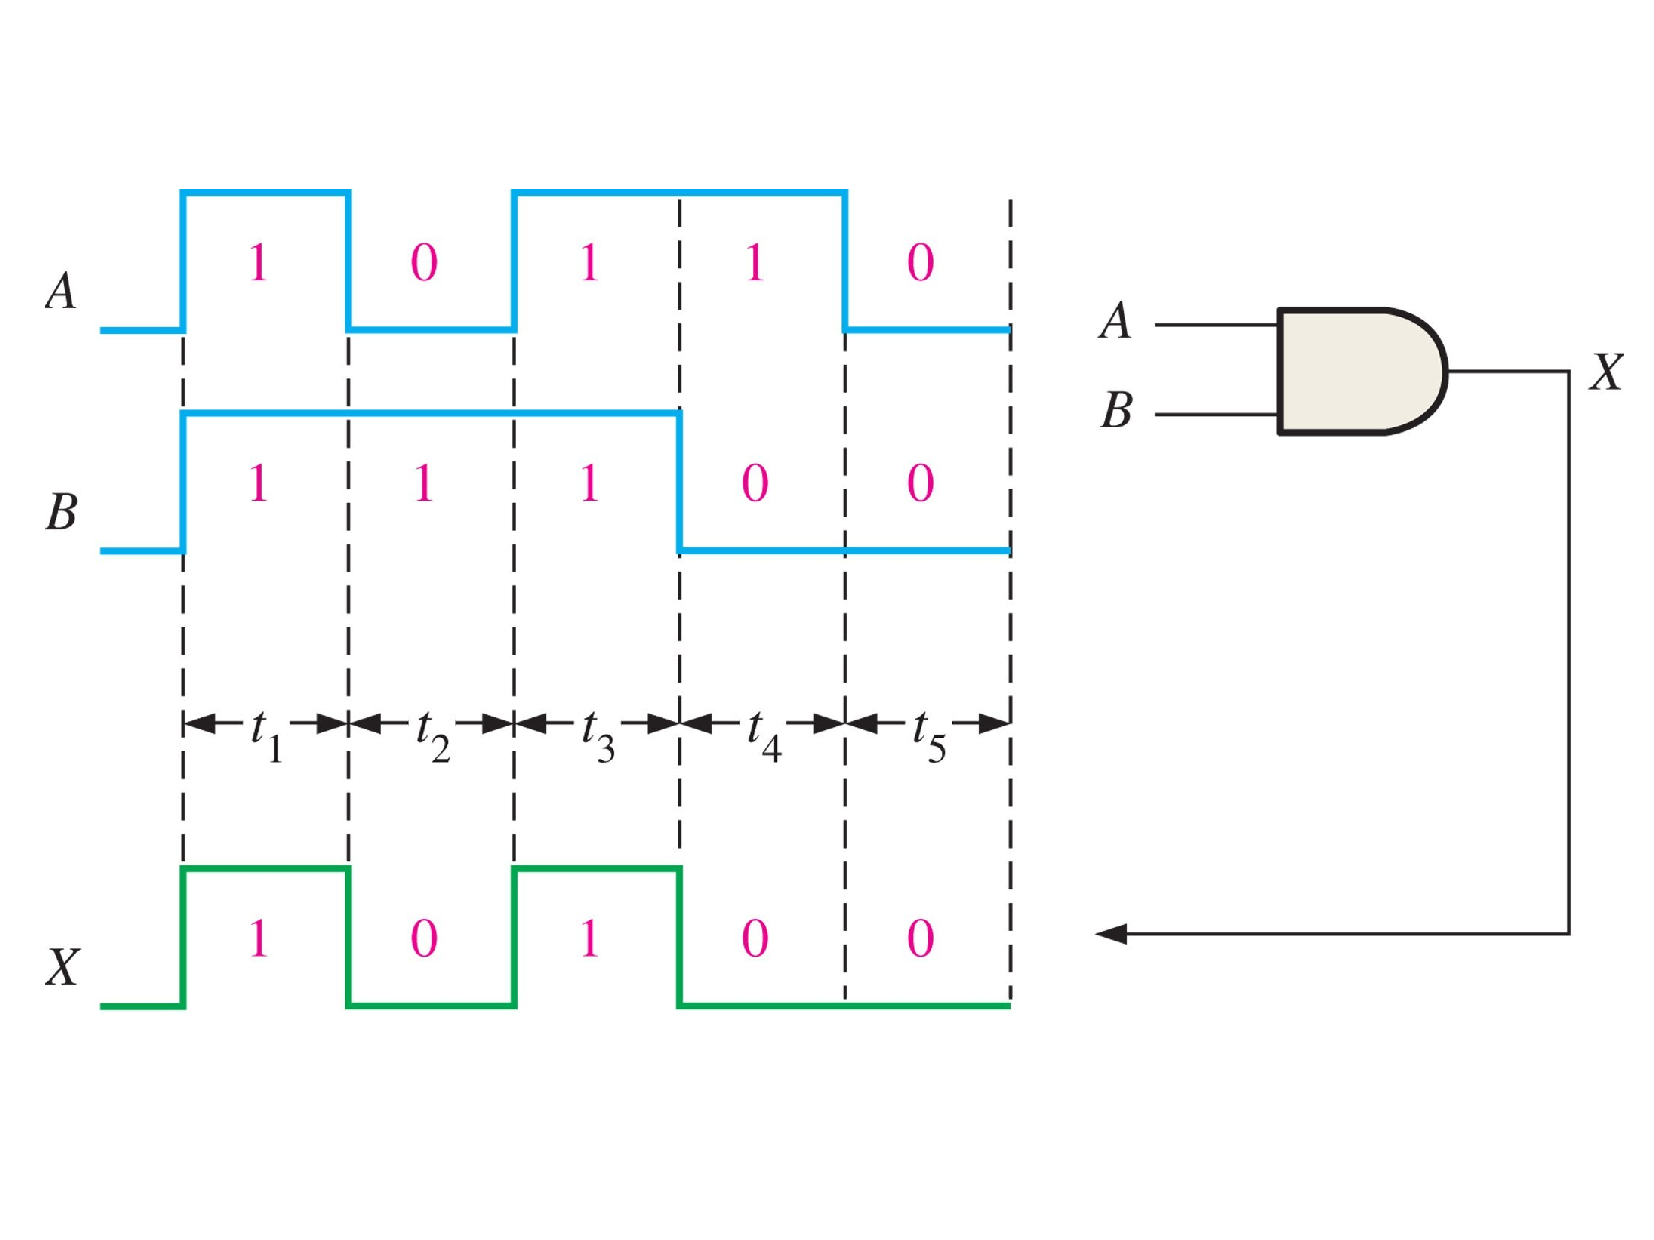
\includegraphics[width=0.8\textwidth]{figures/TimingAnd.pdf}
\caption{\label{fig:and2} Example timing diagram for AND gate.  (Top) Input $A$.  (Middle) Input $B$. (Bottom) $AB$ (A AND B).}
\end{figure}
\end{column}
\end{columns}
\end{frame}

\begin{frame}{Logic Gates}
\textbf{The AND gate:} requires both inputs to be HIGH, for HIGH output. \\ \vspace{0.5cm}
\begin{columns}[T]
\begin{column}{0.5\textwidth}
\begin{itemize}
\item \alert{NOT, $n=1$, $m=1$}
\item \alert{AND, $n$, $m=1$}
\item OR, $n$, $m=1$
\item NAND, $n$, $m=1$
\item NOR, $n=2$, $m=1$
\item XOR, $n=2$, $m=1$
\item XNOR, $n=2$, $m=1$
\end{itemize}
\end{column}
\begin{column}{0.5\textwidth}
\begin{equation}
A ~ AND ~ B = AB
\end{equation}
\end{column}
\end{columns}
\end{frame}

\begin{frame}{Logic Gates}
\textbf{The AND gate:} requires both inputs to be HIGH, for HIGH output. \\ \vspace{0.5cm}
\begin{columns}[T]
\begin{column}{0.5\textwidth}
\begin{itemize}
\item \alert{NOT, $n=1$, $m=1$}
\item \alert{AND, $n$, $m=1$}
\item OR, $n$, $m=1$
\item NAND, $n$, $m=1$
\item NOR, $n=2$, $m=1$
\item XOR, $n=2$, $m=1$
\item XNOR, $n=2$, $m=1$
\end{itemize}
\end{column}
\begin{column}{0.5\textwidth}
\small 
\textbf{In-class exercises:}
\begin{itemize}
\item Using AND as ``enable:'' Develop a circuit that activates an LED circuit every time the clock signal is HIGH, but only if an enable signal is also raised to HIGH.
\item Derive the truth table for a 3-input AND gate.  How many input combinations should there be?
\end{itemize}
\end{column}
\end{columns}
\end{frame}

\begin{frame}{Logic Gates}
\textbf{The AND gate:} requires both inputs to be HIGH, for HIGH output. \\ \vspace{0.5cm}
\begin{columns}[T]
\begin{column}{0.5\textwidth}
\begin{itemize}
\item \alert{NOT, $n=1$, $m=1$}
\item \alert{AND, $n$, $m=1$}
\item OR, $n$, $m=1$
\item NAND, $n$, $m=1$
\item NOR, $n=2$, $m=1$
\item XOR, $n=2$, $m=1$
\item XNOR, $n=2$, $m=1$
\end{itemize}
\end{column}
\begin{column}{0.5\textwidth}
\begin{figure}
\centering
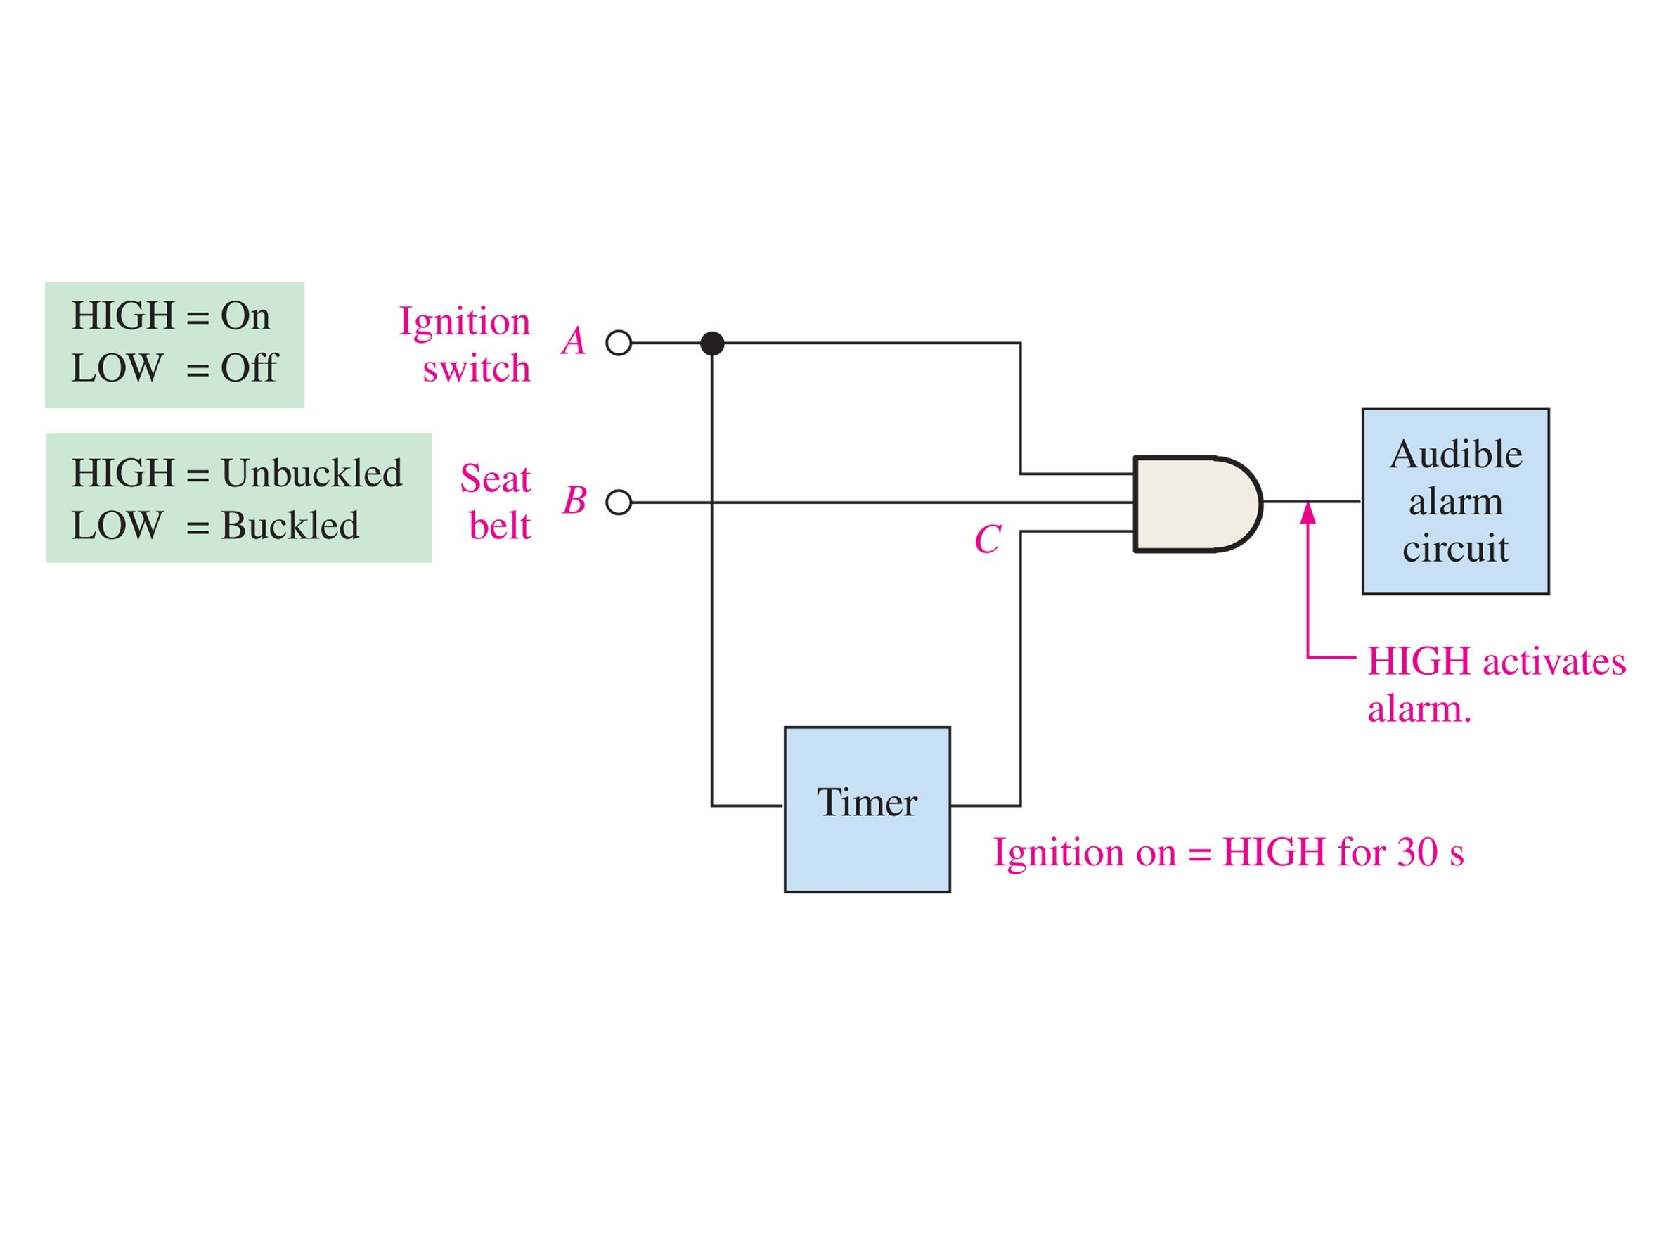
\includegraphics[width=0.9\textwidth,trim=0cm 4cm 0cm 4cm,clip=true]{figures/seat.pdf}
\caption{\label{fig:seat} Example of AND enable plus timing: seatbelt sensor.}
\end{figure}
\end{column}
\end{columns}
\end{frame}

\begin{frame}{Logic Gates}
\textbf{The OR gate:} requires either input to be HIGH, for HIGH output. \\ \vspace{0.5cm}
\begin{columns}[T]
\begin{column}{0.5\textwidth}
\begin{itemize}
\item \alert{NOT, $n=1$, $m=1$}
\item \alert{AND, $n$, $m=1$}
\item \alert{OR, $n$, $m=1$}
\item NAND, $n$, $m=1$
\item NOR, $n=2$, $m=1$
\item XOR, $n=2$, $m=1$
\item XNOR, $n=2$, $m=1$
\end{itemize}
\end{column}
\begin{column}{0.5\textwidth}
\begin{figure}
\centering
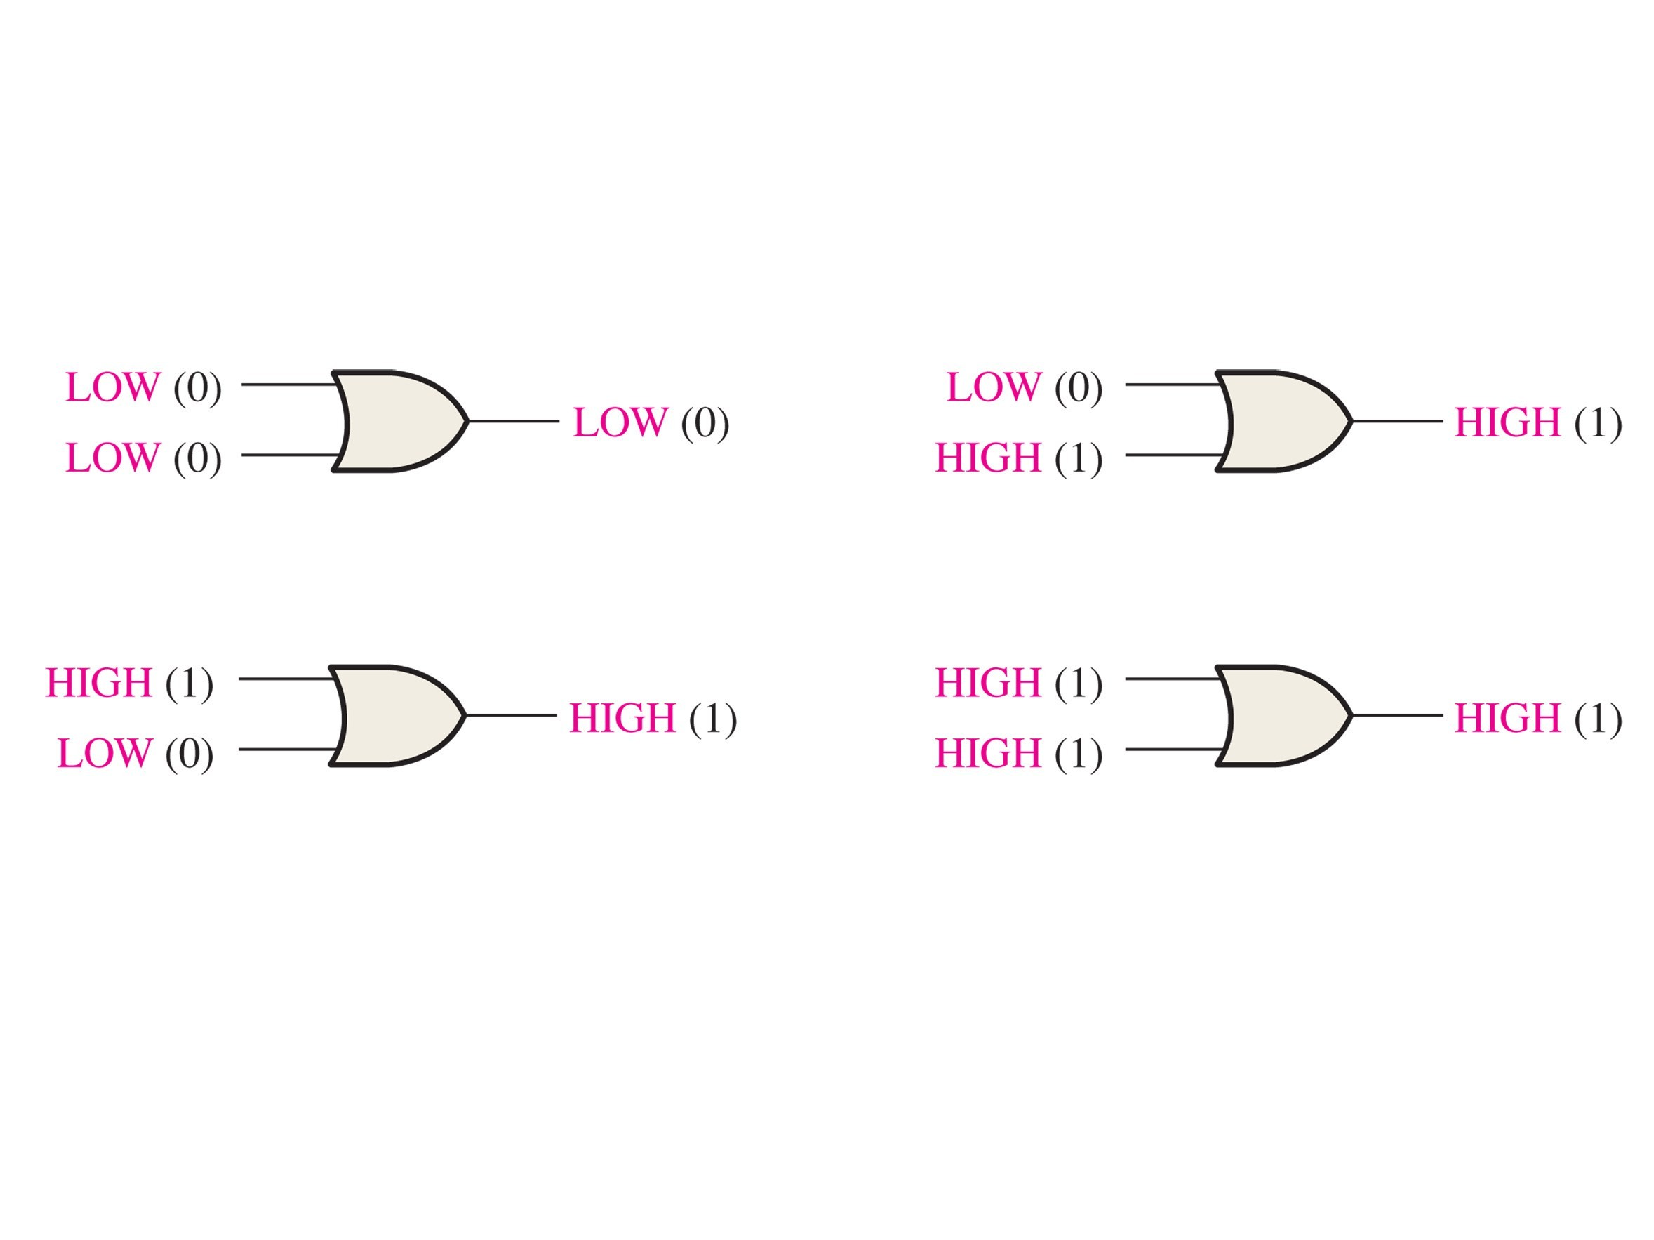
\includegraphics[width=0.8\textwidth,trim=0cm 5cm 0cm 5cm,clip=true]{figures/BasicOR.pdf}
\caption{\label{fig:or} The circuit representation of an OR gate.  Two inputs, one output.}
\end{figure}
\end{column}
\end{columns}
\end{frame}

\begin{frame}{Logic Gates}
\textbf{The OR gate:} requires either input to be HIGH, for HIGH output. \\ \vspace{0.5cm}
\begin{columns}[T]
\begin{column}{0.5\textwidth}
\begin{itemize}
\item \alert{NOT, $n=1$, $m=1$}
\item \alert{AND, $n$, $m=1$}
\item \alert{OR, $n$, $m=1$}
\item NAND, $n$, $m=1$
\item NOR, $n=2$, $m=1$
\item XOR, $n=2$, $m=1$
\item XNOR, $n=2$, $m=1$
\end{itemize}
\end{column}
\begin{column}{0.5\textwidth}
\begin{table}
\begin{tabular}{c c c}
A & B & X \\
1 & 1 & 1 \\
1 & 0 & 1 \\
0 & 1 & 1 \\
0 & 0 & 0
\end{tabular}
\caption{\label{tab:OR} Truth table for OR.}
\end{table}
\end{column}
\end{columns}
\end{frame}

\begin{frame}{Logic Gates}
\textbf{The OR gate:} requires either input to be HIGH, for HIGH output. \\ \vspace{0.5cm}
\begin{columns}[T]
\begin{column}{0.5\textwidth}
\begin{itemize}
\item \alert{NOT, $n=1$, $m=1$}
\item \alert{AND, $n$, $m=1$}
\item \alert{OR, $n$, $m=1$}
\item NAND, $n$, $m=1$
\item NOR, $n=2$, $m=1$
\item XOR, $n=2$, $m=1$
\item XNOR, $n=2$, $m=1$
\end{itemize}
\end{column}
\begin{column}{0.5\textwidth}
\begin{figure}
\centering
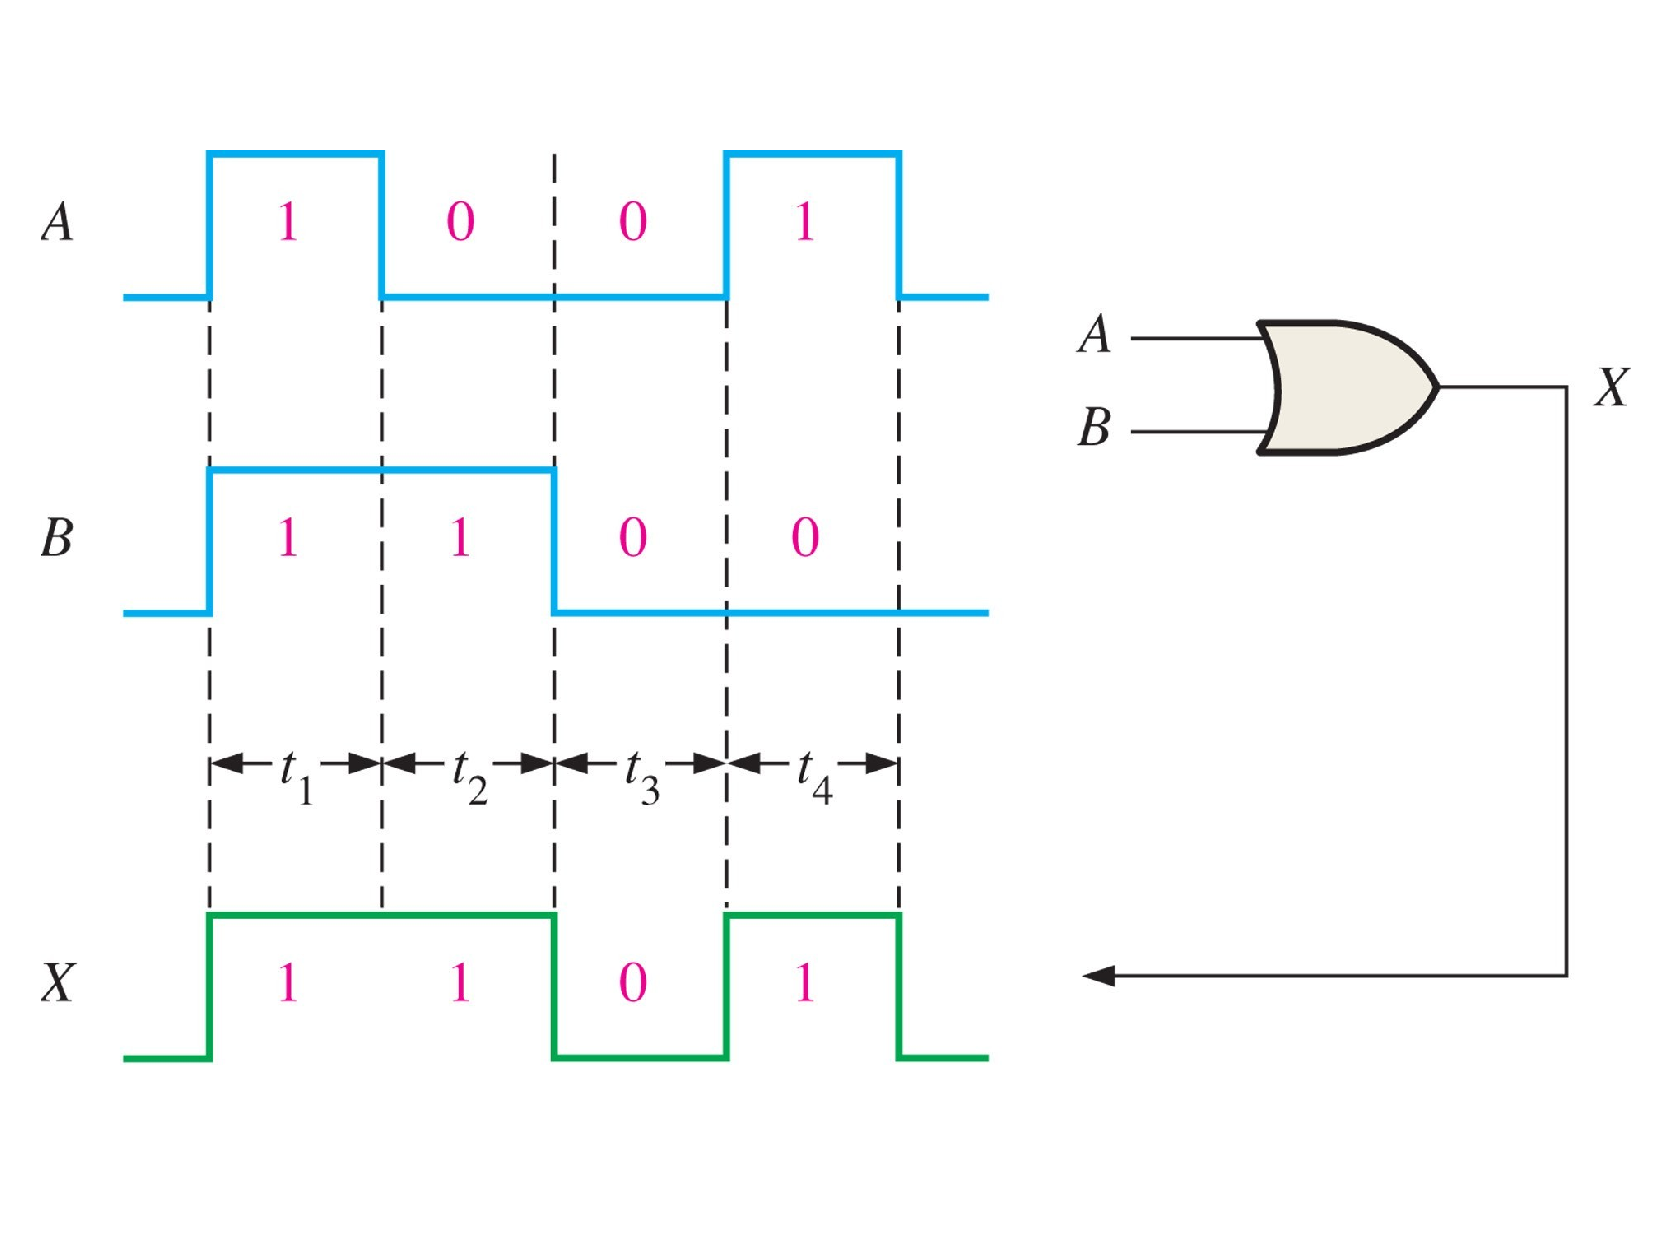
\includegraphics[width=0.8\textwidth]{figures/TimingOr.pdf}
\caption{\label{fig:or2} Example timing diagram for OR gate.  (Top) Input $A$.  (Middle) Input $B$. (Bottom) $A+B$ (A OR B).}
\end{figure}
\end{column}
\end{columns}
\end{frame}

\begin{frame}{Logic Gates}
\textbf{The OR gate:} requires either input to be HIGH, for HIGH output. \\ \vspace{0.5cm}
\begin{columns}[T]
\begin{column}{0.5\textwidth}
\begin{itemize}
\item \alert{NOT, $n=1$, $m=1$}
\item \alert{AND, $n$, $m=1$}
\item \alert{OR, $n$, $m=1$}
\item NAND, $n$, $m=1$
\item NOR, $n=2$, $m=1$
\item XOR, $n=2$, $m=1$
\item XNOR, $n=2$, $m=1$
\end{itemize}
\end{column}
\begin{column}{0.5\textwidth}
\begin{equation}
A ~ OR ~ B = A+B
\end{equation}
\end{column}
\end{columns}
\end{frame}

\begin{frame}{Logic Gates}
\textbf{The OR gate:} requires either input to be HIGH, for HIGH output. \\ \vspace{0.5cm}
\begin{columns}[T]
\begin{column}{0.5\textwidth}
\begin{itemize}
\item \alert{NOT, $n=1$, $m=1$}
\item \alert{AND, $n$, $m=1$}
\item \alert{OR, $n$, $m=1$}
\item NAND, $n$, $m=1$
\item NOR, $n=2$, $m=1$
\item XOR, $n=2$, $m=1$
\item XNOR, $n=2$, $m=1$
\end{itemize}
\end{column}
\begin{column}{0.5\textwidth}
\tiny
\textbf{In-class exercises:}
\begin{itemize}
\item In physics experiments, sometimes we establish a \textit{combinatorial trigger}, sometimes called a coincidence trigger.  Suppose the task of three digital channels is to observe a high-energy particle pass through a detector.  If there is an observation in a channel, it raises HIGH for a time called a \textit{gate time.}
\item Using OR gates, draw a circuit that triggers if \textbf{two of the three} channels observes the particle.  Draw an example of a timing diagram corresponding to a trigger. (The gate time is up to you, it just means that if a channel is HIGH it stays high for at least one gate).
\end{itemize}
\end{column}
\end{columns}
\end{frame}

\begin{frame}{Logic Gates}
\textbf{The NAND gate:} requires \textbf{neither} input to be HIGH for the output to be HIGH \\ \vspace{0.5cm}
\begin{columns}[T]
\begin{column}{0.5\textwidth}
\begin{itemize}
\item \alert{NOT, $n=1$, $m=1$}
\item \alert{AND, $n$, $m=1$}
\item \alert{OR, $n$, $m=1$}
\item \alert{NAND, $n$, $m=1$}
\item NOR, $n=2$, $m=1$
\item XOR, $n=2$, $m=1$
\item XNOR, $n=2$, $m=1$
\end{itemize}
\end{column}
\begin{column}{0.5\textwidth}
\begin{figure}
\centering
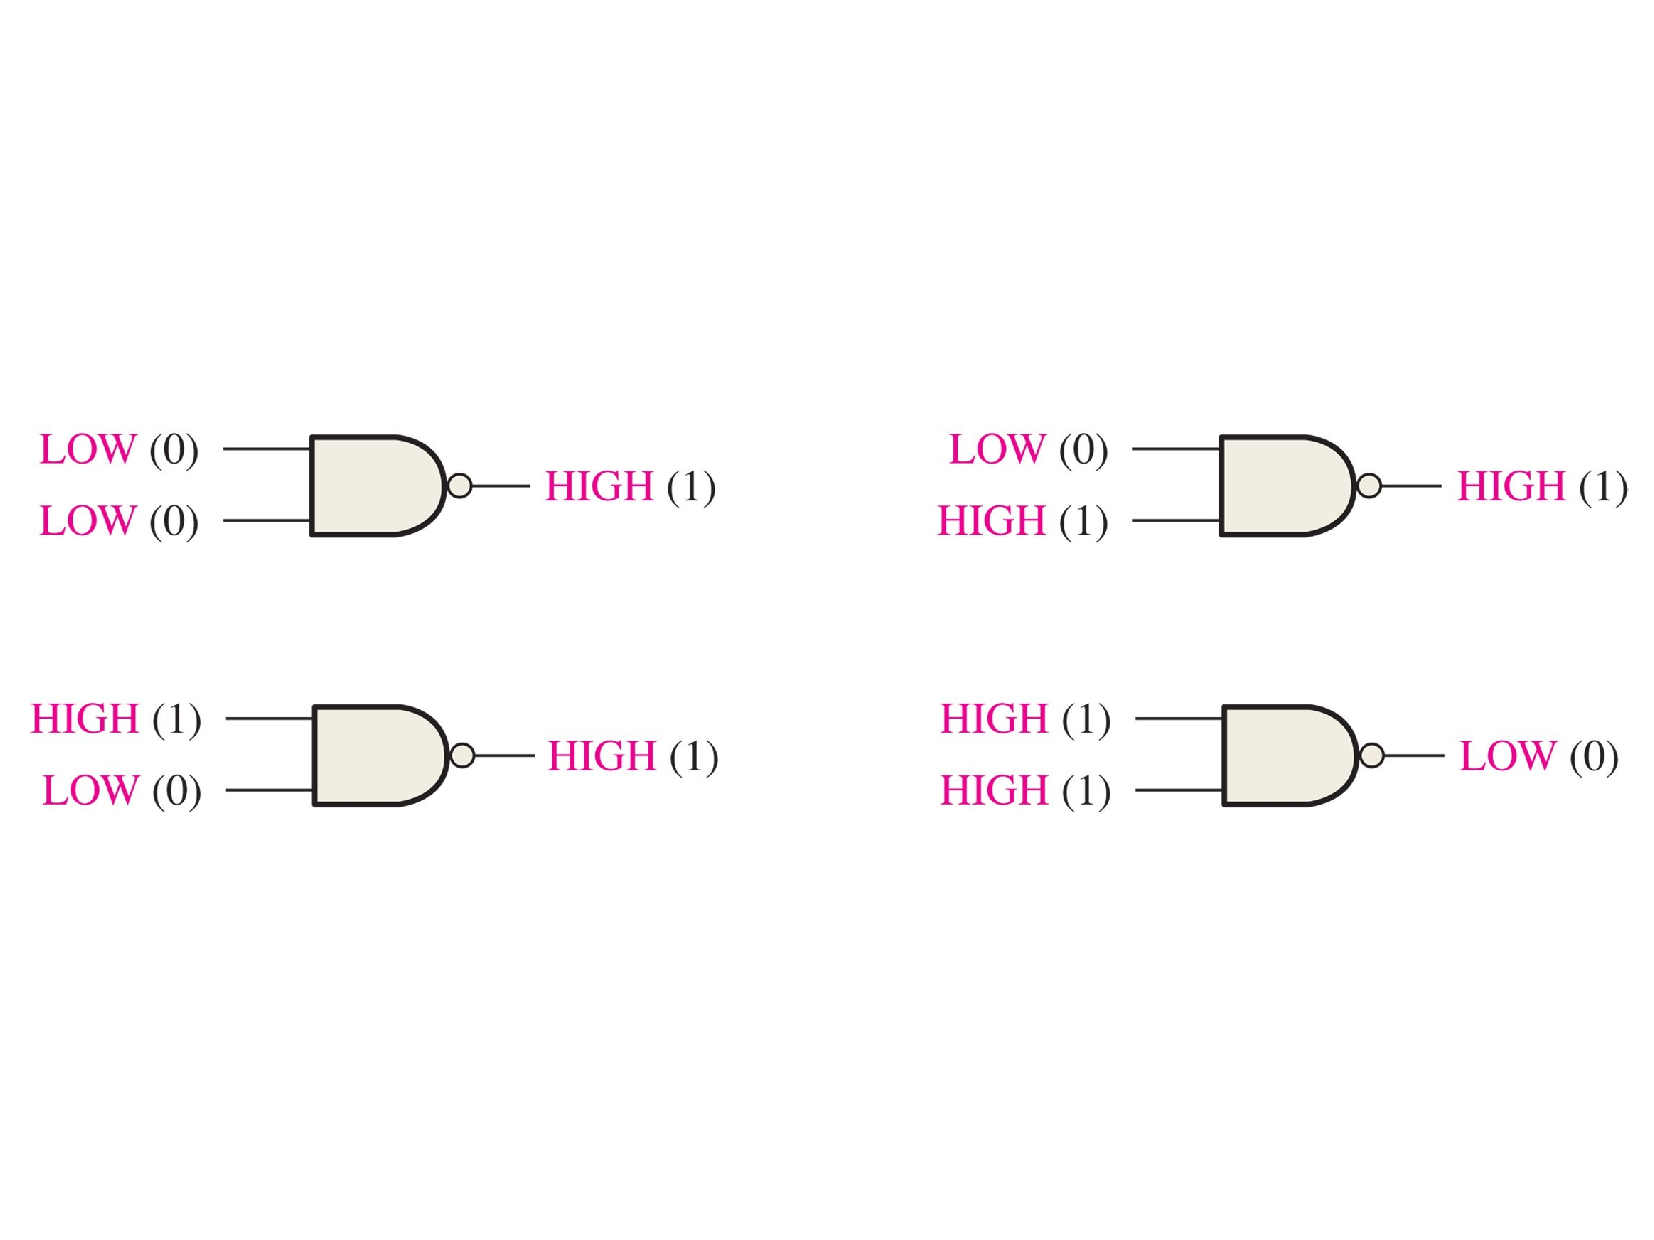
\includegraphics[width=0.7\textwidth]{figures/BasicNAND.pdf}
\caption{\label{fig:nand} The circuit representation of an NAND gate.  Two inputs, one output.}
\end{figure}
\end{column}
\end{columns}
\end{frame}

\begin{frame}{Logic Gates}
\textbf{The NAND gate:} requires \textbf{neither} input to be HIGH for the output to be HIGH \\ \vspace{0.5cm}
\begin{columns}[T]
\begin{column}{0.5\textwidth}
\begin{itemize}
\item \alert{NOT, $n=1$, $m=1$}
\item \alert{AND, $n$, $m=1$}
\item \alert{OR, $n$, $m=1$}
\item \alert{NAND, $n$, $m=1$}
\item NOR, $n=2$, $m=1$
\item XOR, $n=2$, $m=1$
\item XNOR, $n=2$, $m=1$
\end{itemize}
\end{column}
\begin{column}{0.5\textwidth}
\begin{table}
\begin{tabular}{c c c}
A & B & X \\
1 & 1 & 0 \\
1 & 0 & 1 \\
0 & 1 & 1 \\
0 & 0 & 1
\end{tabular}
\caption{\label{tab:NAND} Truth table for NAND.}
\end{table}
\end{column}
\end{columns}
\end{frame}

\begin{frame}{Logic Gates}
\textbf{The NAND gate:} requires \textbf{neither} input to be HIGH for the output to be HIGH \\ \vspace{0.5cm}
\begin{columns}[T]
\begin{column}{0.5\textwidth}
\begin{itemize}
\item \alert{NOT, $n=1$, $m=1$}
\item \alert{AND, $n$, $m=1$}
\item \alert{OR, $n$, $m=1$}
\item \alert{NAND, $n$, $m=1$}
\item NOR, $n=2$, $m=1$
\item XOR, $n=2$, $m=1$
\item XNOR, $n=2$, $m=1$
\end{itemize}
\end{column}
\begin{column}{0.5\textwidth}
\begin{figure}
\centering
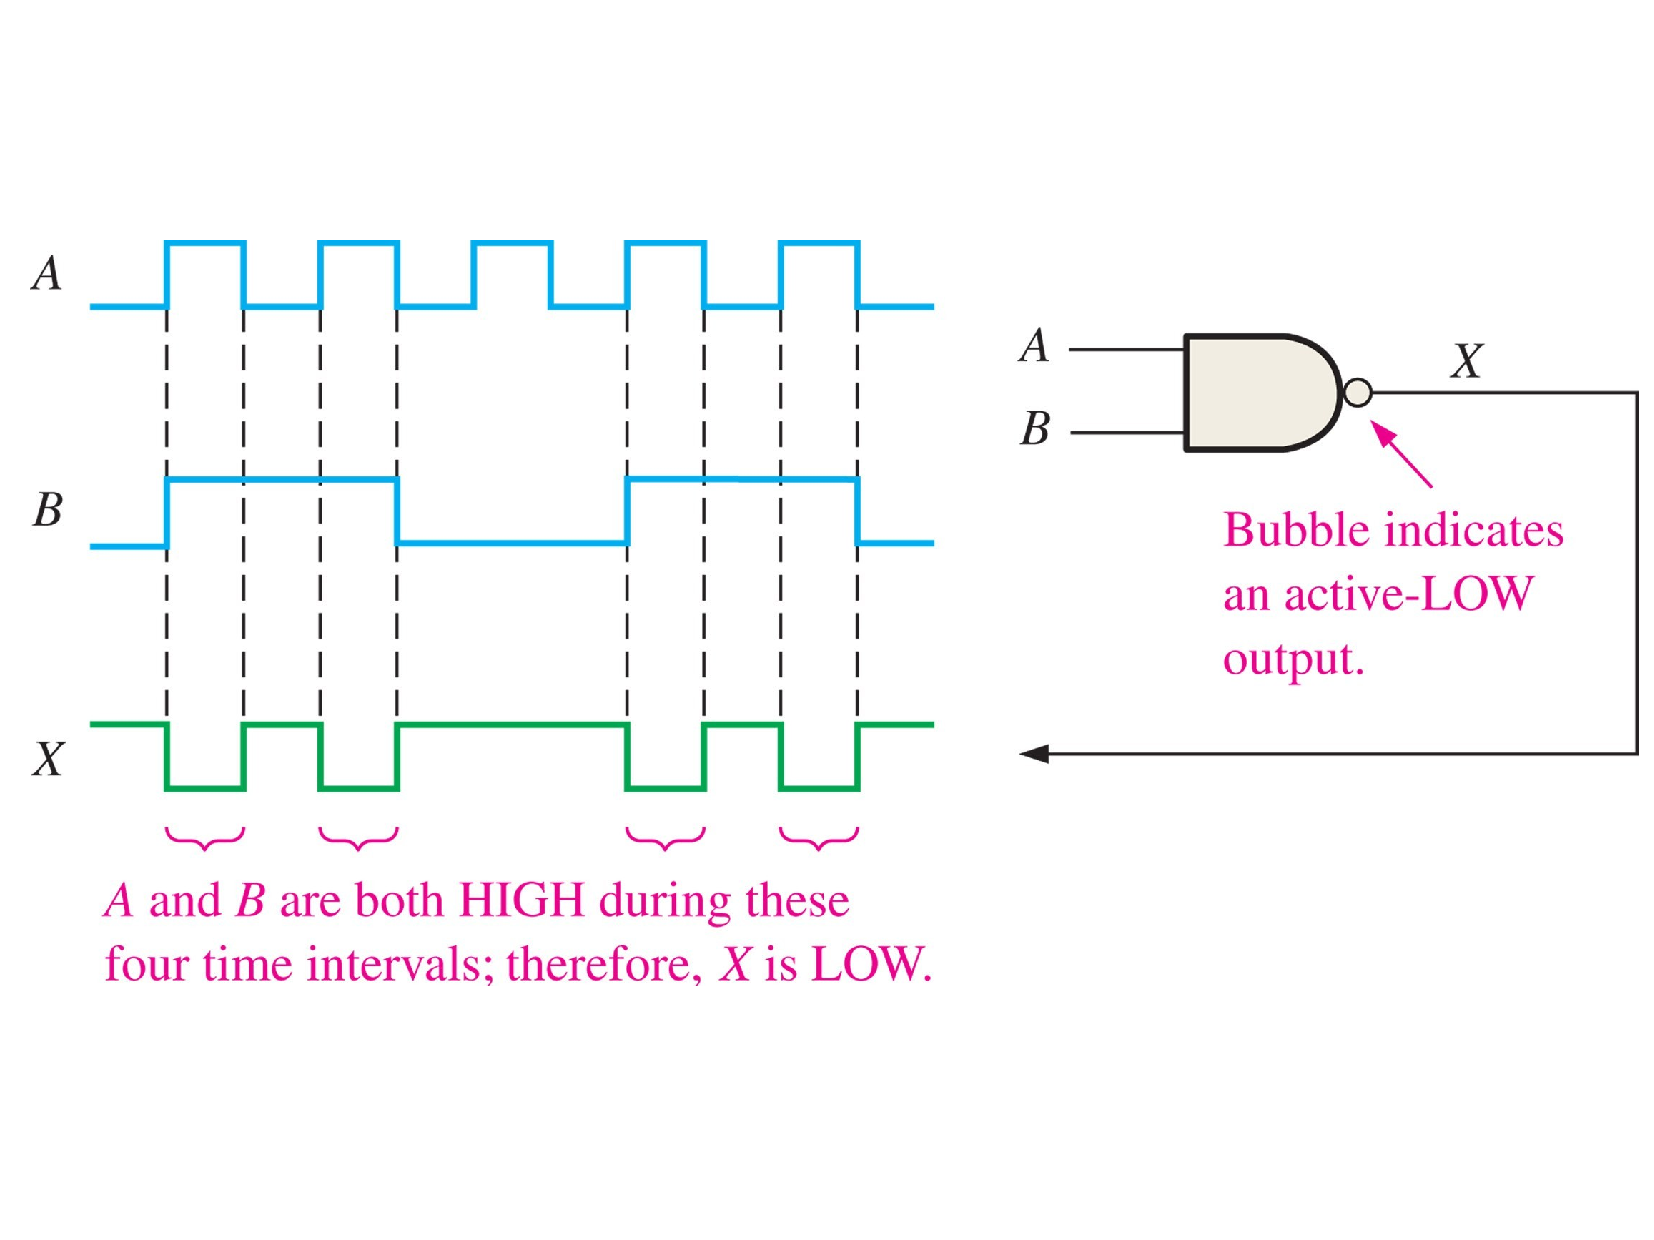
\includegraphics[width=0.8\textwidth]{figures/TimingNand.pdf}
\caption{\label{fig:nand2} Example timing diagram for NAND gate.  (Top) Input $A$.  (Middle) Input $B$. (Bottom) $\overline{AB}$ (A NAND B or NAND AB).}
\end{figure}
\end{column}
\end{columns}
\end{frame}

\begin{frame}{Logic Gates}
\textbf{The NAND gate:} requires \textbf{neither} input to be HIGH for the output to be HIGH \\ \vspace{0.5cm}
\begin{columns}[T]
\begin{column}{0.5\textwidth}
\begin{itemize}
\item \alert{NOT, $n=1$, $m=1$}
\item \alert{AND, $n$, $m=1$}
\item \alert{OR, $n$, $m=1$}
\item \alert{NAND, $n$, $m=1$}
\item NOR, $n=2$, $m=1$
\item XOR, $n=2$, $m=1$
\item XNOR, $n=2$, $m=1$
\end{itemize}
\end{column}
\begin{column}{0.5\textwidth}
\begin{equation}
A ~ NAND ~ B = \overline{AB}
\end{equation}
Note: have you started to pick up the notation here?  The bar is like complex conjugation, or the \textit{\textbf{compliment}} of the signal.
\end{column}
\end{columns}
\end{frame}

\begin{frame}{Logic Gates}
\textbf{The NAND gate:} requires \textbf{neither} input to be HIGH for the output to be HIGH \\ \vspace{0.5cm}
\begin{columns}[T]
\begin{column}{0.5\textwidth}
\begin{itemize}
\item \alert{NOT, $n=1$, $m=1$}
\item \alert{AND, $n$, $m=1$}
\item \alert{OR, $n$, $m=1$}
\item \alert{NAND, $n$, $m=1$}
\item NOR, $n=2$, $m=1$
\item XOR, $n=2$, $m=1$
\item XNOR, $n=2$, $m=1$
\end{itemize}
\end{column}
\begin{column}{0.5\textwidth}
\small
\textbf{In-class exercises:}
\begin{itemize}
\item A certain fluid pump has a display that shows sensor information from two pairs of pipes, pair A and pair B.  The sensors are raised HIGH if no fluid is flowing through a pipe, and there is one sensor per pipe.
\end{itemize}
\end{column}
\end{columns}
\end{frame}

\begin{frame}{Logic Gates}
\textbf{The NAND gate:} requires \textbf{neither} input to be HIGH for the output to be HIGH \\ \vspace{0.5cm}
\begin{columns}[T]
\begin{column}{0.5\textwidth}
\begin{itemize}
\item \alert{NOT, $n=1$, $m=1$}
\item \alert{AND, $n$, $m=1$}
\item \alert{OR, $n$, $m=1$}
\item \alert{NAND, $n$, $m=1$}
\item NOR, $n=2$, $m=1$
\item XOR, $n=2$, $m=1$
\item XNOR, $n=2$, $m=1$
\end{itemize}
\end{column}
\begin{column}{0.5\textwidth}
\small
\textbf{In-class exercises:}
\begin{itemize}
\item Design a system using NAND gates that produces three output signals: one LOW if neither pipe in pair A has fluid flowing, one LOW if neither pipe in pair B has fluid flowing, and one LOW if neither pair has fluid flowing.  Create a timing diagram that shows pair A turning off, then pair B.
\end{itemize}
\end{column}
\end{columns}
\end{frame}

\begin{frame}{Logic Gates}
\textbf{The NAND gate:} requires \textbf{neither} input to be HIGH for the output to be HIGH \\ \vspace{0.5cm}
\begin{columns}[T]
\begin{column}{0.5\textwidth}
\begin{itemize}
\item \alert{NOT, $n=1$, $m=1$}
\item \alert{AND, $n$, $m=1$}
\item \alert{OR, $n$, $m=1$}
\item \alert{NAND, $n$, $m=1$}
\item NOR, $n=2$, $m=1$
\item XOR, $n=2$, $m=1$
\item XNOR, $n=2$, $m=1$
\end{itemize}
\end{column}
\begin{column}{0.5\textwidth}
\small
\textbf{In-class exercises:}
\begin{itemize}
\item Create an OR gate with NAND and NOT gates. a) 2-input version 3) 3-input version.
\item Create an AND gate with NAND and NOT gates. a) 2-input version 3) 3-input version.
\end{itemize}
\end{column}
\end{columns}
\end{frame}

\begin{frame}{Logic Gates}
\textbf{The NOR gate:} requires \textbf{both} inputs to be LOW for the output to be HIGH \\ \vspace{0.5cm}
\begin{columns}[T]
\begin{column}{0.5\textwidth}
\begin{itemize}
\item \alert{NOT, $n=1$, $m=1$}
\item \alert{AND, $n$, $m=1$}
\item \alert{OR, $n$, $m=1$}
\item \alert{NAND, $n$, $m=1$}
\item \alert{NOR, $n=2$, $m=1$}
\item XOR, $n=2$, $m=1$
\item XNOR, $n=2$, $m=1$
\end{itemize}
\end{column}
\begin{column}{0.5\textwidth}
\begin{figure}
\centering
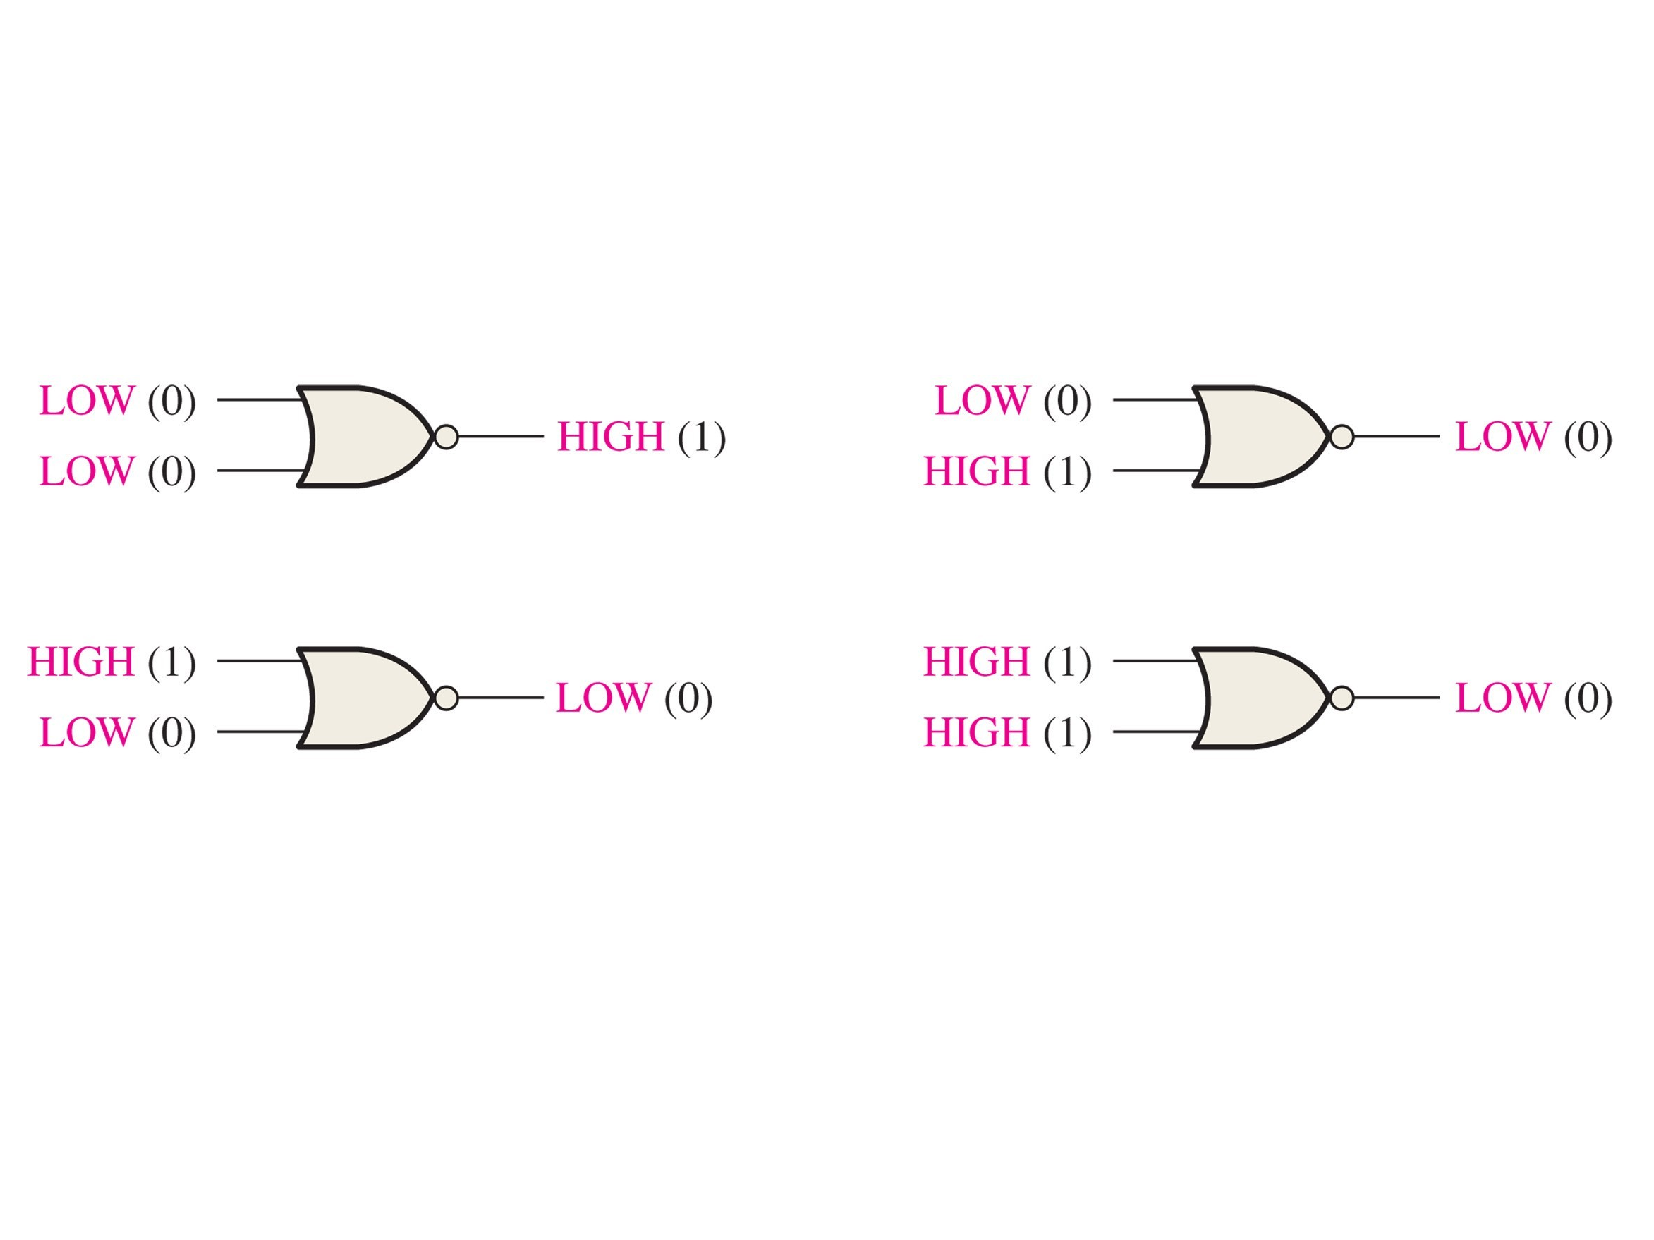
\includegraphics[width=0.8\textwidth,trim=0cm 2cm 0cm 2cm,clip=true]{figures/BasicNOR.pdf}
\caption{\label{fig:nor} The circuit representation of an NOR gate.  Two inputs, one output.}
\end{figure}
\end{column}
\end{columns}
\end{frame}

\begin{frame}{Logic Gates}
\textbf{The NOR gate:} requires \textbf{both} inputs to be LOW for the output to be HIGH \\ \vspace{0.5cm}
\begin{columns}[T]
\begin{column}{0.5\textwidth}
\begin{itemize}
\item \alert{NOT, $n=1$, $m=1$}
\item \alert{AND, $n$, $m=1$}
\item \alert{OR, $n$, $m=1$}
\item \alert{NAND, $n$, $m=1$}
\item \alert{NOR, $n=2$, $m=1$}
\item XOR, $n=2$, $m=1$
\item XNOR, $n=2$, $m=1$
\end{itemize}
\end{column}
\begin{column}{0.5\textwidth}
\begin{table}
\begin{tabular}{c c c}
A & B & X \\
1 & 1 & 0 \\
1 & 0 & 0 \\
0 & 1 & 0 \\
0 & 0 & 1
\end{tabular}
\caption{\label{tab:NOR} Truth table for NOR.}
\end{table}
\end{column}
\end{columns}
\end{frame}

\begin{frame}{Logic Gates}
\textbf{The NOR gate:} requires \textbf{both} inputs to be LOW for the output to be HIGH \\ \vspace{0.5cm}
\begin{columns}[T]
\begin{column}{0.5\textwidth}
\begin{itemize}
\item \alert{NOT, $n=1$, $m=1$}
\item \alert{AND, $n$, $m=1$}
\item \alert{OR, $n$, $m=1$}
\item \alert{NAND, $n$, $m=1$}
\item \alert{NOR, $n=2$, $m=1$}
\item XOR, $n=2$, $m=1$
\item XNOR, $n=2$, $m=1$
\end{itemize}
\end{column}
\begin{column}{0.5\textwidth}
\begin{figure}
\centering
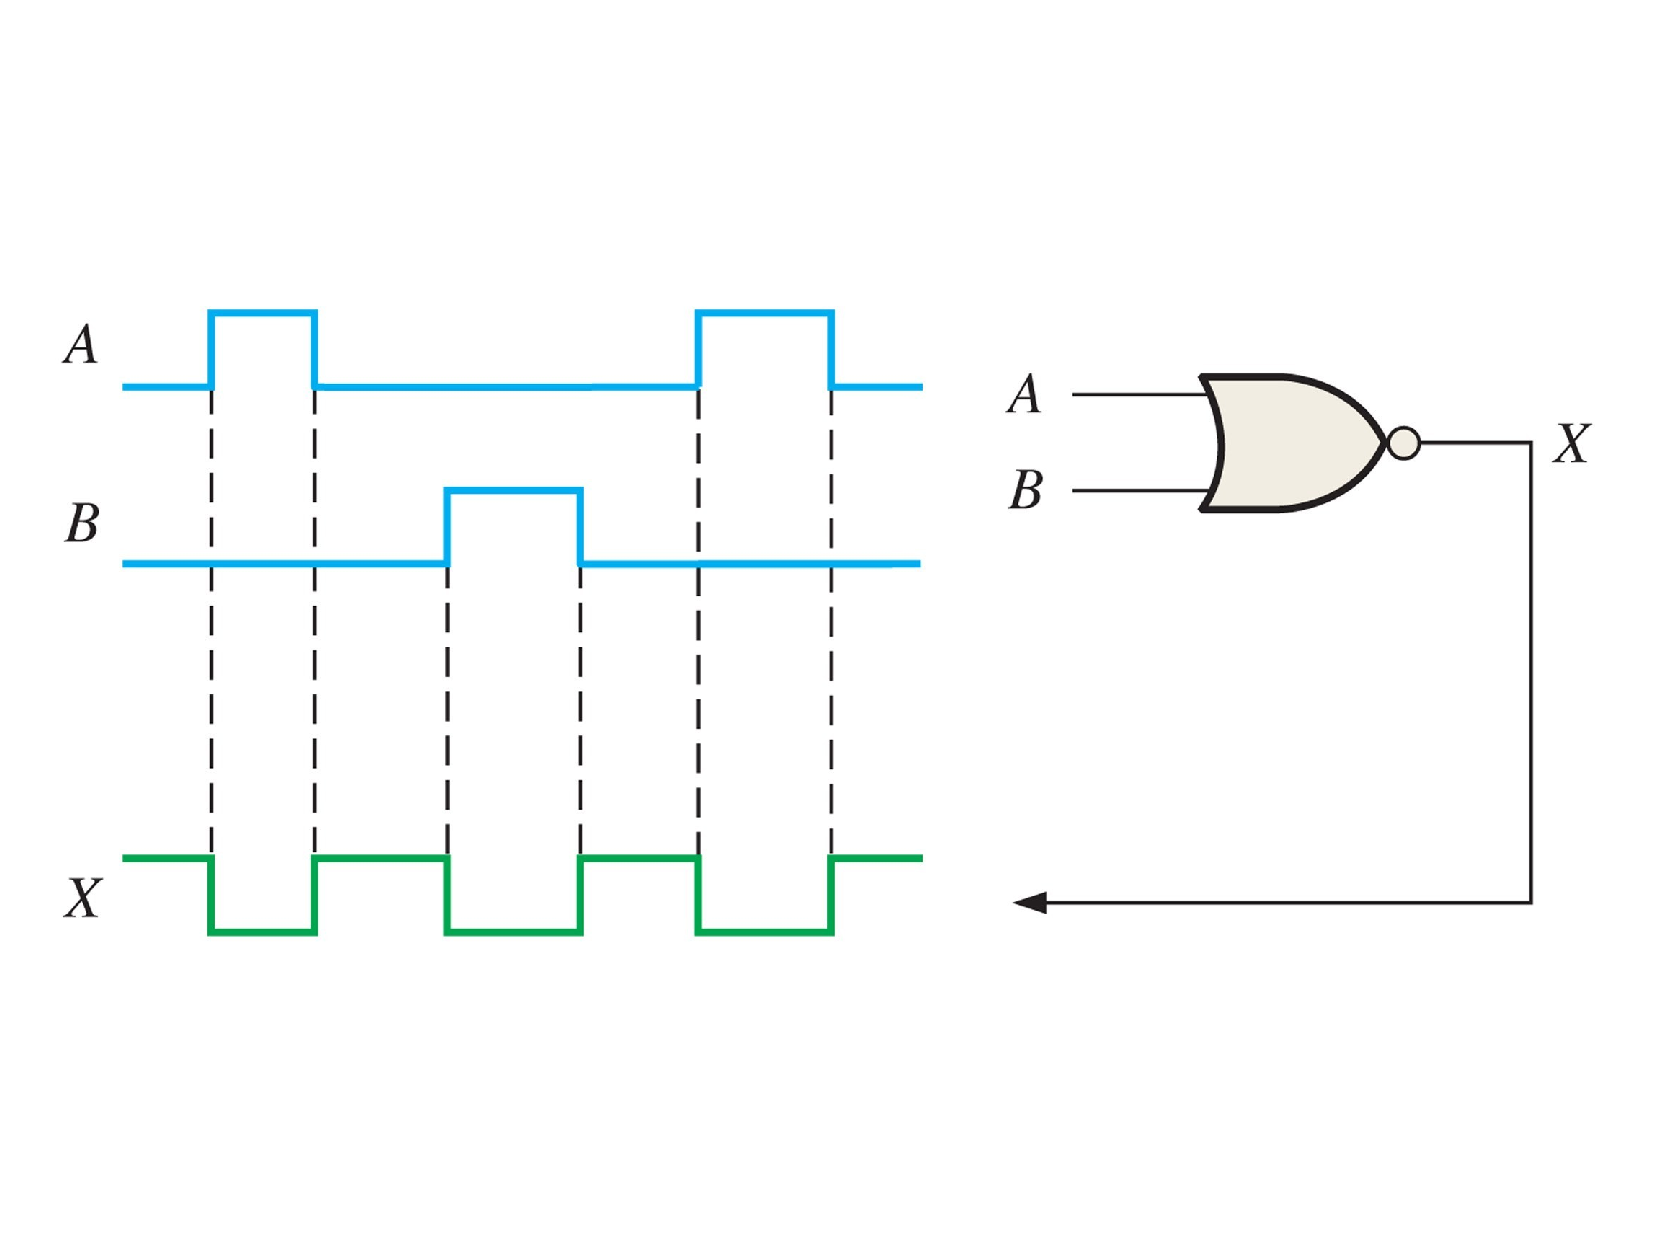
\includegraphics[width=0.8\textwidth]{figures/TimingNor.pdf}
\caption{\label{fig:nor2} Example timing diagram for NOR gate.  (Top) Input $A$.  (Middle) Input $B$. (Bottom) $\overline{A+B}$ (A NOR B or NOR AB).}
\end{figure}
\end{column}
\end{columns}
\end{frame}

\begin{frame}{Logic Gates}
\textbf{The NOR gate:} requires \textbf{both} inputs to be LOW for the output to be HIGH \\ \vspace{0.5cm}
\begin{columns}[T]
\begin{column}{0.5\textwidth}
\begin{itemize}
\item \alert{NOT, $n=1$, $m=1$}
\item \alert{AND, $n$, $m=1$}
\item \alert{OR, $n$, $m=1$}
\item \alert{NAND, $n$, $m=1$}
\item \alert{NOR, $n=2$, $m=1$}
\item XOR, $n=2$, $m=1$
\item XNOR, $n=2$, $m=1$
\end{itemize}
\end{column}
\begin{column}{0.5\textwidth}
\begin{equation}
A ~ NOR ~ B = \overline{A+B}
\end{equation}
\end{column}
\end{columns}
\end{frame}

\begin{frame}{Logic Gates}
\textbf{The NOR gate:} requires \textbf{both} inputs to be LOW for the output to be HIGH \\ \vspace{0.5cm}
\begin{columns}[T]
\begin{column}{0.5\textwidth}
\begin{itemize}
\item \alert{NOT, $n=1$, $m=1$}
\item \alert{AND, $n$, $m=1$}
\item \alert{OR, $n$, $m=1$}
\item \alert{NAND, $n$, $m=1$}
\item \alert{NOR, $n=2$, $m=1$}
\item XOR, $n=2$, $m=1$
\item XNOR, $n=2$, $m=1$
\end{itemize}
\end{column}
\begin{column}{0.5\textwidth}
\textbf{In-class exercises:}
\begin{itemize}
\item Create a NOR gate from a NAND gate and inverters.  a) 2-input version b) 3-input version.  Verify with either a timing diagram or truth table.
\end{itemize}
\end{column}
\end{columns}
\end{frame}

\begin{frame}{Logic Gates}
\textbf{The NOR gate:} requires \textbf{both} inputs to be LOW for the output to be HIGH \\ \vspace{0.5cm}
\begin{columns}[T]
\begin{column}{0.5\textwidth}
\begin{itemize}
\item \alert{NOT, $n=1$, $m=1$}
\item \alert{AND, $n$, $m=1$}
\item \alert{OR, $n$, $m=1$}
\item \alert{NAND, $n$, $m=1$}
\item \alert{NOR, $n=2$, $m=1$}
\item XOR, $n=2$, $m=1$
\item XNOR, $n=2$, $m=1$
\end{itemize}
\end{column}
\begin{column}{0.5\textwidth}
\tiny
\textbf{In-class exercise (from the text, this one is cool)}
\begin{itemize}
\item As part of an aircraft's functional monitoring system, a circuit is required to indicate the status of the landing gears prior to landing.  A green LED display turns on if all three gears are properly extended when the gear-down switch has been activated in preparation for landing.  A red LED display turns on if any of the gears fail to extend properly prior to landing.  When a landing gear is extended, its sensor produces a LOW voltage.  When a landing gear is retracted, its sensor produces a HIGH voltage.  Implement a circuit to meet this requirement.
\end{itemize}
\alert{To solve this problem, let's have a quick aside as to how LED's (light emitting diodes) work...}
\end{column}
\end{columns}
\end{frame}

\begin{frame}{Logic Gates}
\textbf{LED - light emitting diode.}  What's a diode?  What is a transistor?  One kind of transistor is a p-n-p junction, or a n-p-n junction:
\begin{figure}
\centering
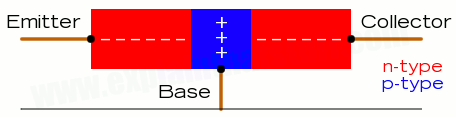
\includegraphics[width=0.45\textwidth]{figures/transistor2.png}
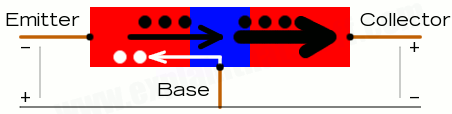
\includegraphics[width=0.45\textwidth]{figures/transistor3.png}
\caption{\label{fig:trans1} One kind of transistor is the sandwich of semiconductors.}
\end{figure}
\end{frame}

\begin{frame}{Logic Gates}
\textbf{LED - light emitting diode.}  What's a diode?  Like a transistor, minus one layer.  Diodes will only conduct in one direction.
\begin{figure}
\centering
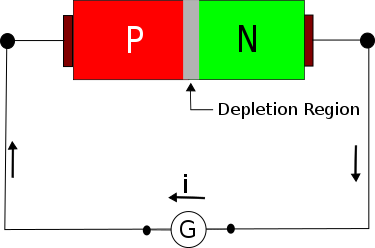
\includegraphics[width=0.45\textwidth]{figures/diode.png}
\caption{\label{fig:diode} A diode is a sandwich of only two layers of semiconductor rather than three.}
\end{figure}
\end{frame}

\begin{frame}{Logic Gates}
\textbf{LED - light emitting diode.}  What's a diode?  Like a transistor, minus one layer.  Diodes will only conduct in one direction.
\begin{figure}
\centering
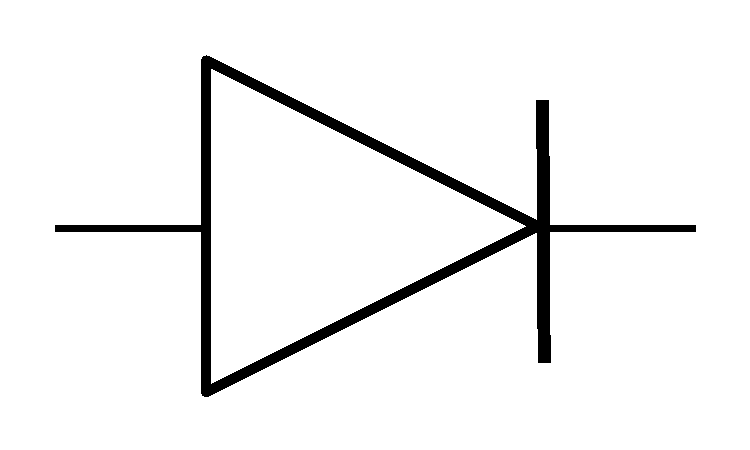
\includegraphics[width=0.45\textwidth]{figures/Diode.pdf}
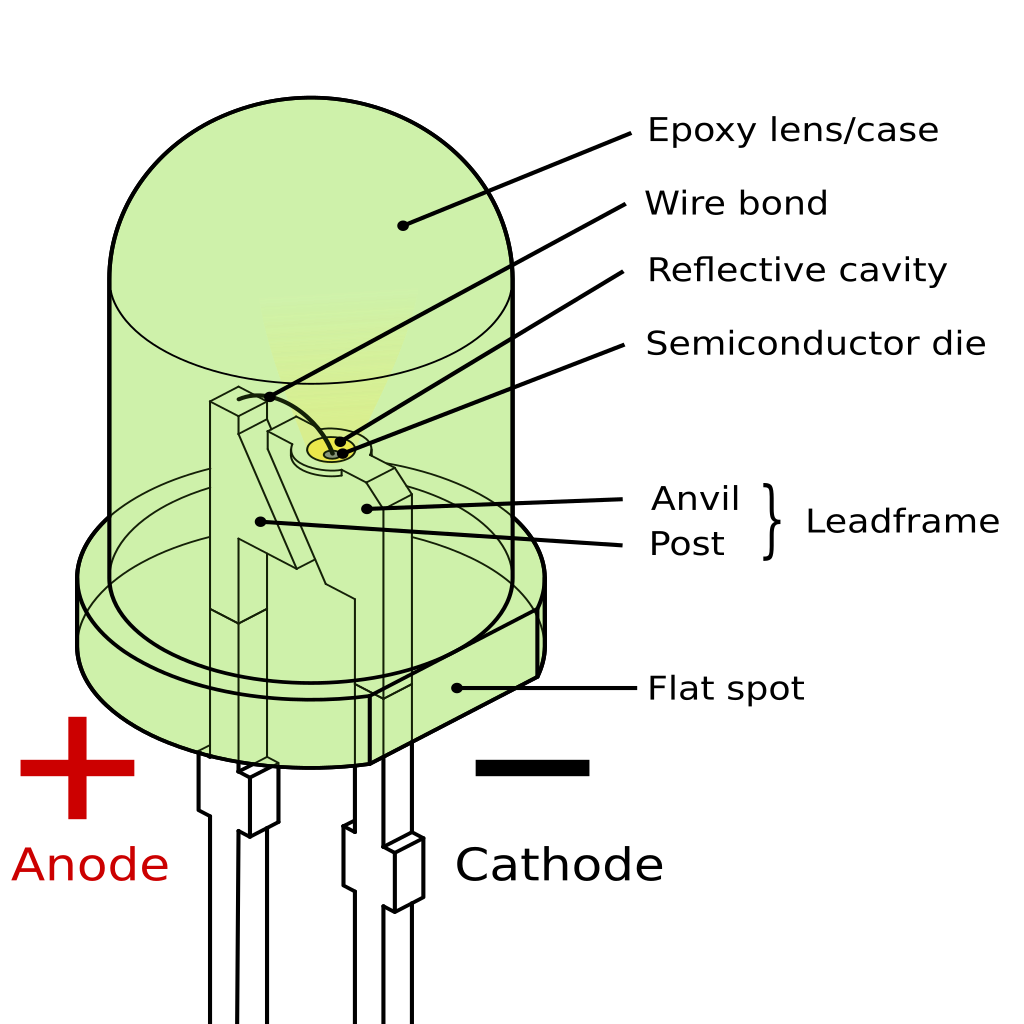
\includegraphics[width=0.45\textwidth]{figures/LED.png}
\caption{\label{fig:diode2} (Left) The symbol for a diode.  Current flows towards the flat line. (Right) Some diodes emit visible photons when conducting electricity.}
\end{figure}
\end{frame}

\begin{frame}{Logic Gates}
\begin{figure}
\centering
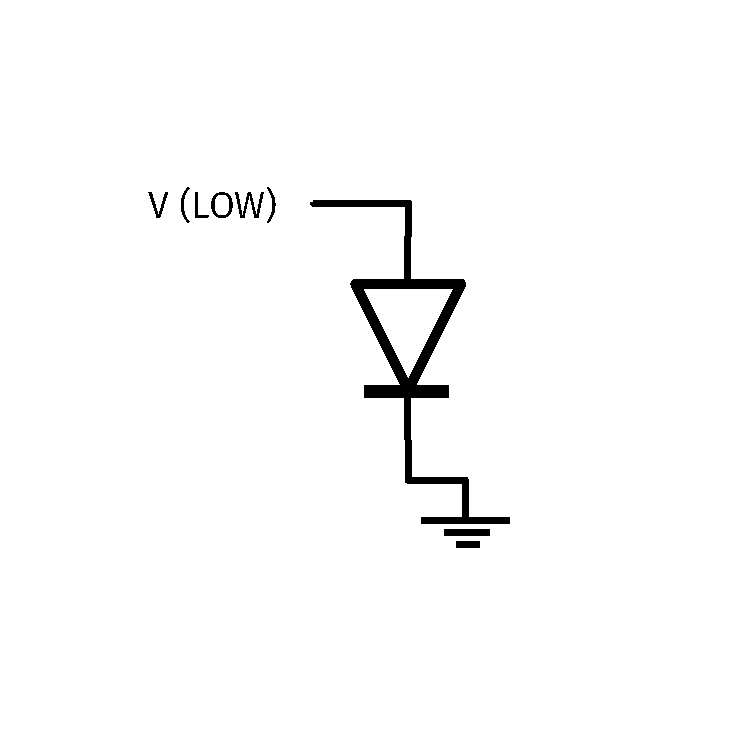
\includegraphics[width=0.35\textwidth,trim=1cm 3cm 1cm 3cm,clip=true]{figures/GreenLEDOff.pdf}
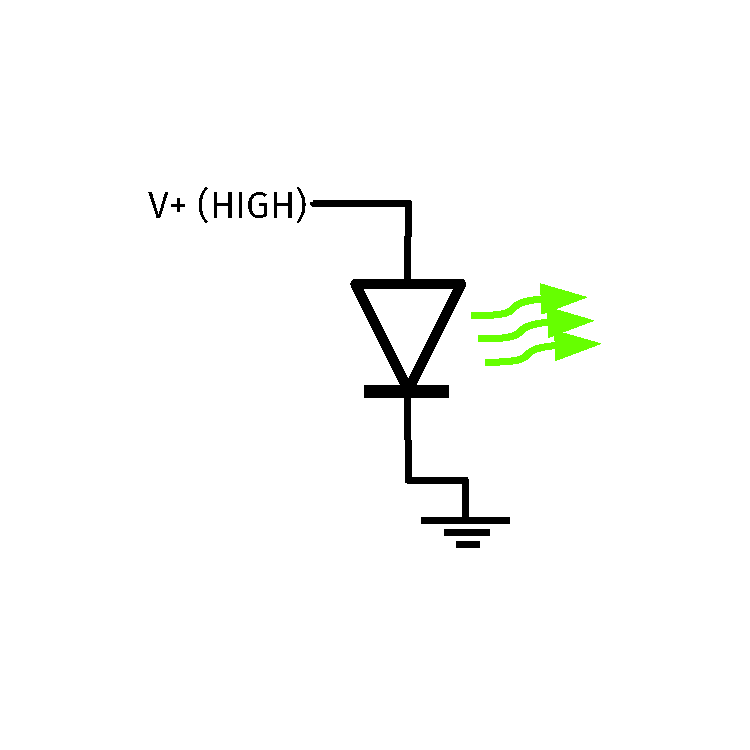
\includegraphics[width=0.35\textwidth,trim=1cm 3cm 1cm 3cm,clip=true]{figures/GreenLEDOn.pdf} \\
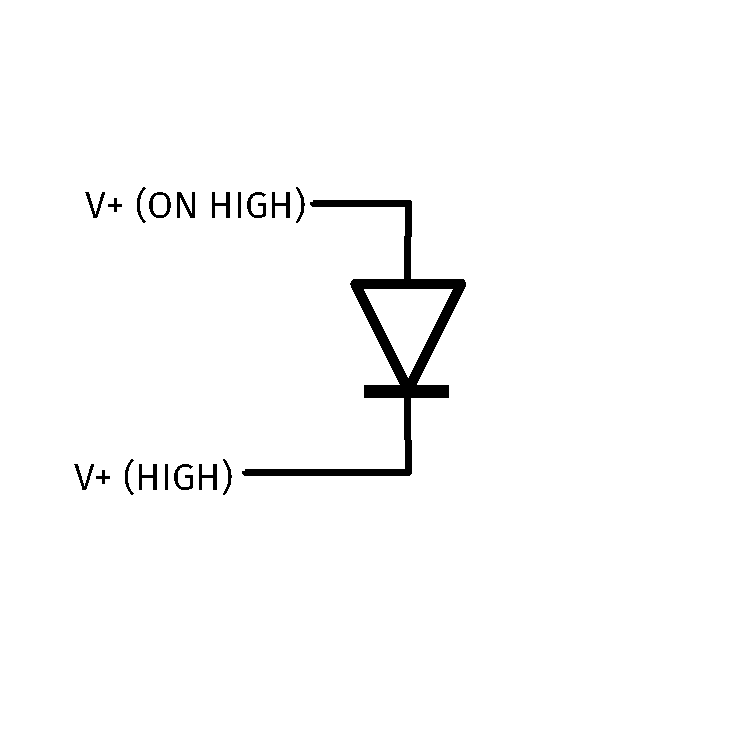
\includegraphics[width=0.35\textwidth,trim=1cm 3cm 1cm 3cm,clip=true]{figures/RedLEDOff.pdf}
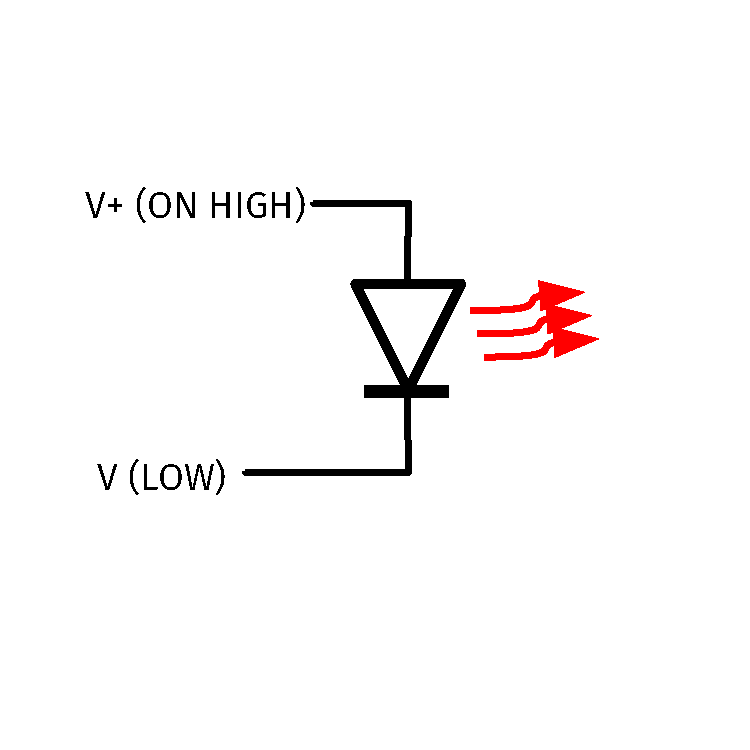
\includegraphics[width=0.35\textwidth,trim=1cm 3cm 1cm 3cm,clip=true]{figures/RedLEDOn.pdf}
\caption{\label{fig:diode3} \small (Upper left): The green LED is held off by a LOW signal, no voltage gradient. (Upper right) The green LED is activated by a HIGH signal, a voltage gradient.  (Lower left): The red LED is held off by a HIGH signal, no voltage gradient.  (Lower right): The red LED is activated by a LOW signal, a voltage gradient.}
\end{figure}
\end{frame}

\begin{frame}{Logic Gates}
\textbf{The NOR gate:} requires \textbf{both} inputs to be LOW for the output to be HIGH \\ \vspace{0.5cm}
\begin{columns}[T]
\begin{column}{0.5\textwidth}
\begin{itemize}
\item \alert{NOT, $n=1$, $m=1$}
\item \alert{AND, $n$, $m=1$}
\item \alert{OR, $n$, $m=1$}
\item \alert{NAND, $n$, $m=1$}
\item \alert{NOR, $n=2$, $m=1$}
\item XOR, $n=2$, $m=1$
\item XNOR, $n=2$, $m=1$
\end{itemize}
\end{column}
\begin{column}{0.5\textwidth}
\tiny
\textbf{So now we can solve this problem:}
\begin{itemize}
\item As part of an aircraft's functional monitoring system, a circuit is required to indicate the status of the landing gears prior to landing.  A green LED display turns on if all three gears are properly extended when the gear-down switch has been activated in preparation for landing.  A red LED display turns on if any of the gears fail to extend properly prior to landing.  When a landing gear is extended, its sensor produces a LOW voltage.  When a landing gear is retracted, its sensor produces a HIGH voltage.  Implement a circuit to meet this requirement.
\end{itemize}
\end{column}
\end{columns}
\end{frame}

\begin{frame}{Logic Gates}
\textbf{The XOR gate:} requires \textbf{exactly one} input to be HIGH for the output to be HIGH \\ \vspace{0.5cm}
\begin{columns}[T]
\begin{column}{0.5\textwidth}
\begin{itemize}
\item \alert{NOT, $n=1$, $m=1$}
\item \alert{AND, $n$, $m=1$}
\item \alert{OR, $n$, $m=1$}
\item \alert{NAND, $n$, $m=1$}
\item \alert{NOR, $n=2$, $m=1$}
\item \alert{XOR, $n=2$, $m=1$}
\item XNOR, $n=2$, $m=1$
\end{itemize}
\end{column}
\begin{column}{0.5\textwidth}
\begin{figure}
\centering
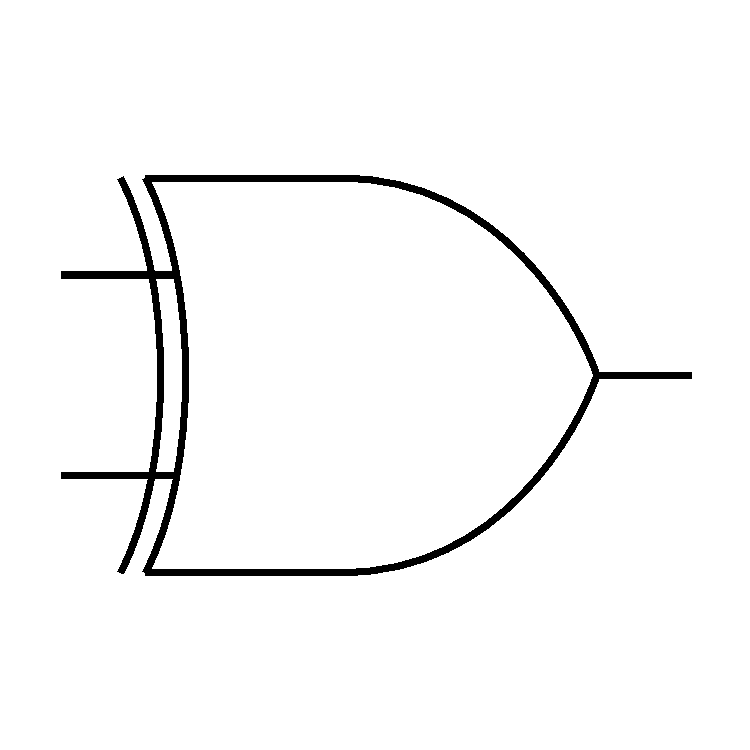
\includegraphics[width=0.8\textwidth,trim=0cm 2cm 0cm 2cm,clip=true]{figures/BasicXOR.pdf}
\caption{\label{fig:xor} The circuit representation of an XOR gate.  Two inputs, one output.}
\end{figure}
\end{column}
\end{columns}
\end{frame}


\begin{frame}{Logic Gates}
\textbf{The XOR gate:} requires \textbf{exactly one} input to be HIGH for the output to be HIGH \\ \vspace{0.5cm}
\begin{columns}[T]
\begin{column}{0.5\textwidth}
\begin{itemize}
\item \alert{NOT, $n=1$, $m=1$}
\item \alert{AND, $n$, $m=1$}
\item \alert{OR, $n$, $m=1$}
\item \alert{NAND, $n$, $m=1$}
\item \alert{NOR, $n=2$, $m=1$}
\item \alert{XOR, $n=2$, $m=1$}
\item XNOR, $n=2$, $m=1$
\end{itemize}
\end{column}
\begin{column}{0.5\textwidth}
\begin{table}
\begin{tabular}{c c c}
A & B & X \\
1 & 1 & 0 \\
1 & 0 & 1 \\
0 & 1 & 1 \\
0 & 0 & 0
\end{tabular}
\caption{\label{tab:XOR} Truth table for XOR.}
\end{table}
\end{column}
\end{columns}
\end{frame}

\begin{frame}{Logic Gates}
\textbf{The XOR gate:} requires \textbf{exactly one} input to be HIGH for the output to be HIGH \\ \vspace{0.5cm}
\begin{columns}[T]
\begin{column}{0.5\textwidth}
\begin{itemize}
\item \alert{NOT, $n=1$, $m=1$}
\item \alert{AND, $n$, $m=1$}
\item \alert{OR, $n$, $m=1$}
\item \alert{NAND, $n$, $m=1$}
\item \alert{NOR, $n=2$, $m=1$}
\item \alert{XOR, $n=2$, $m=1$}
\item XNOR, $n=2$, $m=1$
\end{itemize}
\end{column}
\begin{column}{0.5\textwidth}
\begin{figure}
\centering
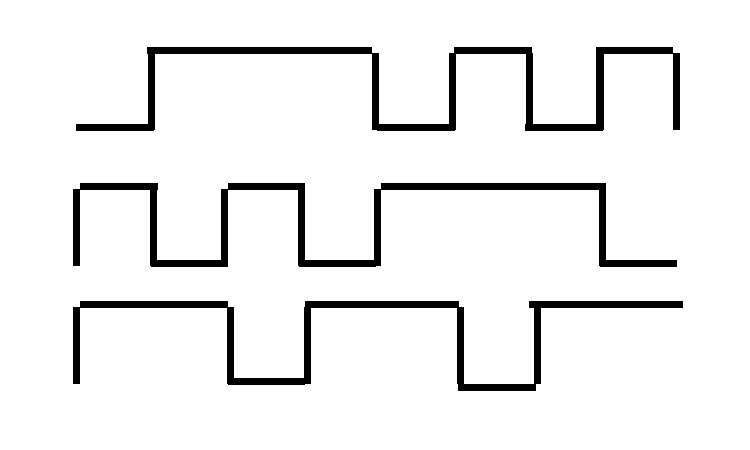
\includegraphics[width=0.8\textwidth]{figures/TimingXor.pdf}
\caption{\label{fig:xor2} Example timing diagram for XOR gate.  (Top) Input $A$.  (Middle) Input $B$. (Bottom) Output}
\end{figure}
\end{column}
\end{columns}
\end{frame}

\begin{frame}{Logic Gates}
\textbf{The XNOR gate:} requires \textbf{both} inputs to be HIGH or LOW for the output to be HIGH \\ \vspace{0.5cm}
\begin{columns}[T]
\begin{column}{0.5\textwidth}
\begin{itemize}
\item \alert{NOT, $n=1$, $m=1$}
\item \alert{AND, $n$, $m=1$}
\item \alert{OR, $n$, $m=1$}
\item \alert{NAND, $n$, $m=1$}
\item \alert{NOR, $n=2$, $m=1$}
\item \alert{XOR, $n=2$, $m=1$}
\item \alert{XNOR, $n=2$, $m=1$}
\end{itemize}
\end{column}
\begin{column}{0.5\textwidth}
\begin{figure}
\centering
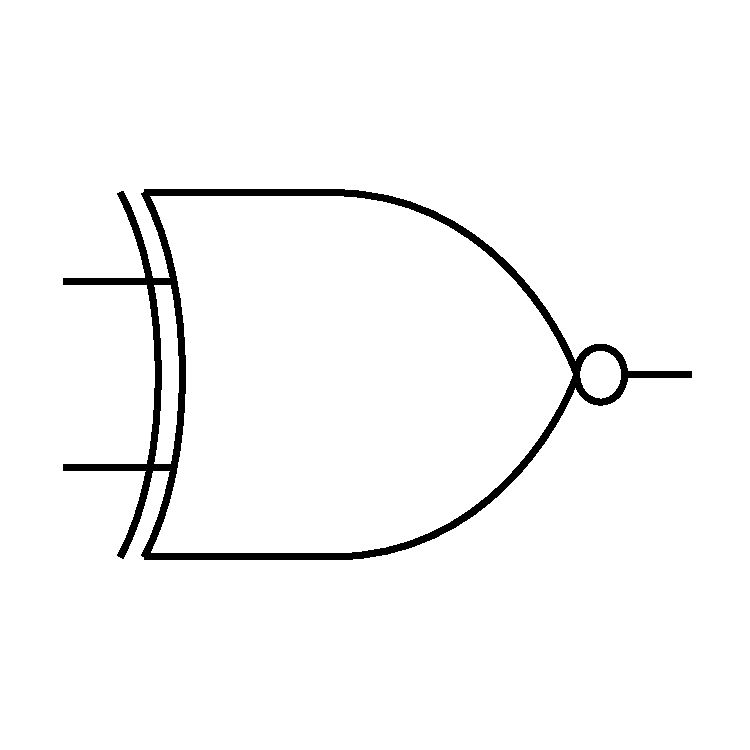
\includegraphics[width=0.8\textwidth,trim=0cm 2cm 0cm 2cm,clip=true]{figures/BasicXNOR.pdf}
\caption{\label{fig:xnor} The circuit representation of an XNOR gate.  Two inputs, one output.}
\end{figure}
\end{column}
\end{columns}
\end{frame}

\begin{frame}{Logic Gates}
\textbf{The XNOR gate:} requires \textbf{both} inputs to be HIGH or LOW for the output to be HIGH \\ \vspace{0.5cm}
\begin{columns}[T]
\begin{column}{0.5\textwidth}
\begin{itemize}
\item \alert{NOT, $n=1$, $m=1$}
\item \alert{AND, $n$, $m=1$}
\item \alert{OR, $n$, $m=1$}
\item \alert{NAND, $n$, $m=1$}
\item \alert{NOR, $n=2$, $m=1$}
\item \alert{XOR, $n=2$, $m=1$}
\item \alert{XNOR, $n=2$, $m=1$}
\end{itemize}
\end{column}
\begin{column}{0.5\textwidth}
\begin{table}
\begin{tabular}{c c c}
A & B & X \\
1 & 1 & 1 \\
1 & 0 & 0 \\
0 & 1 & 0 \\
0 & 0 & 1
\end{tabular}
\caption{\label{tab:XNOR} Truth table for XNOR.}
\end{table}
\end{column}
\end{columns}
\end{frame}

\begin{frame}{Logic Gates}
\textbf{The XNOR gate:} requires \textbf{both} inputs to be HIGH or LOW for the output to be HIGH \\ \vspace{0.5cm}
\begin{columns}[T]
\begin{column}{0.5\textwidth}
\begin{itemize}
\item \alert{NOT, $n=1$, $m=1$}
\item \alert{AND, $n$, $m=1$}
\item \alert{OR, $n$, $m=1$}
\item \alert{NAND, $n$, $m=1$}
\item \alert{NOR, $n=2$, $m=1$}
\item \alert{XOR, $n=2$, $m=1$}
\item \alert{XNOR, $n=2$, $m=1$}
\end{itemize}
\end{column}
\begin{column}{0.5\textwidth}
\begin{figure}
\centering
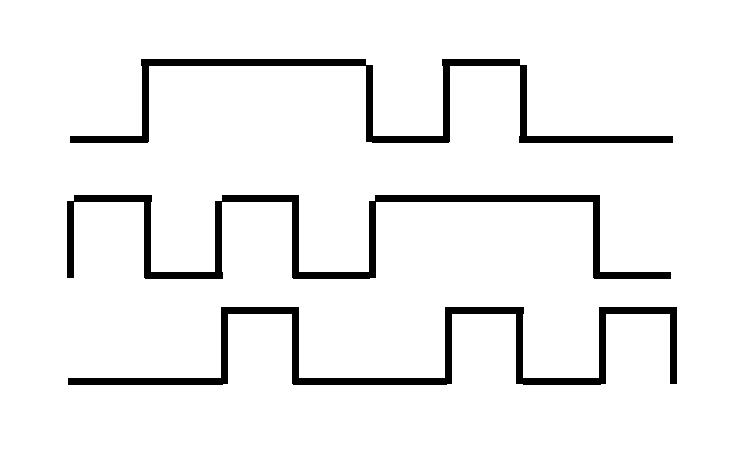
\includegraphics[width=0.8\textwidth]{figures/TimingXnor.pdf}
\caption{\label{fig:xnor2} Example timing diagram for XNOR gate.  (Top) Input $A$.  (Middle) Input $B$. (Bottom) Output}
\end{figure}
\end{column}
\end{columns}
\end{frame}

\begin{frame}{Logic Gates}
\textbf{The NOR gate:} requires \textbf{both} inputs to be LOW for the output to be HIGH \\ \vspace{0.5cm}
\begin{columns}[T]
\begin{column}{0.5\textwidth}
\begin{itemize}
\item \alert{NOT, $n=1$, $m=1$}
\item \alert{AND, $n$, $m=1$}
\item \alert{OR, $n$, $m=1$}
\item \alert{NAND, $n$, $m=1$}
\item \alert{NOR, $n=2$, $m=1$}
\item \alert{XOR, $n=2$, $m=1$}
\item \alert{XNOR, $n=2$, $m=1$}
\end{itemize}
\end{column}
\begin{column}{0.5\textwidth}
\tiny
\textbf{In-class exercises:}
\begin{itemize}
\item Show that an XOR gate is a two-bit adder, neglecting the carry bit.
\item Create an 2-bit adder from XOR and AND gates.
\end{itemize}
\end{column}
\end{columns}
\end{frame}

\begin{frame}{Logic Gates}
\textbf{The NOR gate:} requires \textbf{both} inputs to be LOW for the output to be HIGH \\ \vspace{0.5cm}
\begin{columns}[T]
\begin{column}{0.5\textwidth}
\begin{itemize}
\item \alert{NOT, $n=1$, $m=1$}
\item \alert{AND, $n$, $m=1$}
\item \alert{OR, $n$, $m=1$}
\item \alert{NAND, $n$, $m=1$}
\item \alert{NOR, $n=2$, $m=1$}
\item \alert{XOR, $n=2$, $m=1$}
\item \alert{XNOR, $n=2$, $m=1$}
\end{itemize}
\end{column}
\begin{column}{0.5\textwidth}
\begin{figure}
\centering
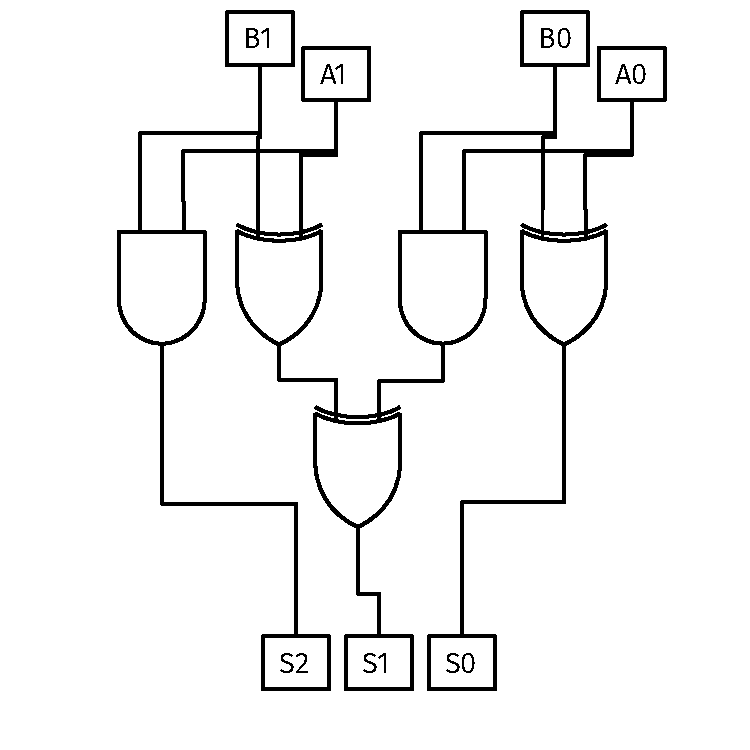
\includegraphics[width=0.8\textwidth]{figures/TwoBitAdder.pdf}
\caption{\label{fig:add} Example of a circuit that adds two-bit digital numbers.}
\end{figure}
\end{column}
\end{columns}
\end{frame}

\begin{frame}{Logic Gates}
\textbf{The NOR gate:} requires \textbf{both} inputs to be LOW for the output to be HIGH \\ \vspace{0.5cm}
\begin{columns}[T]
\begin{column}{0.5\textwidth}
\begin{itemize}
\item \alert{NOT, $n=1$, $m=1$}
\item \alert{AND, $n$, $m=1$}
\item \alert{OR, $n$, $m=1$}
\item \alert{NAND, $n$, $m=1$}
\item \alert{NOR, $n=2$, $m=1$}
\item \alert{XOR, $n=2$, $m=1$}
\item \alert{XNOR, $n=2$, $m=1$}
\end{itemize}
\end{column}
\begin{column}{0.5\textwidth}
\tiny
\textbf{In-class exercises:}
\begin{itemize}
\item Create an 8-bit adder from XOR and AND gates.
\item Account for all-possible carry bits...
\end{itemize}
\end{column}
\end{columns}
\end{frame}

\section{Conclusion}

\begin{frame}{Unit 2.1 Summary - Theoretical Logic Gates, and Operations}
\textbf{Reading: DF Chapter 3-4 (Moodle)}
\begin{enumerate}
\item Logic Gates
\begin{itemize}
\item Circuit diagram
\item Truth table
\item Timing diagram
\item Boolean logic
\end{itemize}
\item \alert{Boolean algebra I}
\item IC Circuits, \textbf{data sheets}
\item \alert{Boolean algebra II}
\end{enumerate}
\end{frame}

\end{document}
